% ============================================================
%  Inside BERT: Architecture, Pre-training, and Fine-tuning
%  CSE Technical Report — Bangladesh University of Engineering
%  and Technology (BUET)
% ============================================================

\documentclass[12pt, a4paper]{article}

% ---- Encoding & Fonts ----------------------------------------
\usepackage[T1]{fontenc}
\usepackage[utf8]{inputenc}
\usepackage{lmodern}
\usepackage{microtype}          % Improved typography

% ---- Page Layout ---------------------------------------------
\usepackage[
  a4paper,
  top=2.5cm, bottom=2.5cm,
  left=2.5cm, right=2.5cm,
  headheight=14pt
]{geometry}

% ---- Mathematics ---------------------------------------------
\usepackage{amsmath, amssymb, amsthm}
\usepackage{mathtools}
\usepackage{bm}                 % Bold math symbols

% ---- Graphics & Figures --------------------------------------
\usepackage{graphicx}
\graphicspath{{figures/}}
\usepackage{float}
\usepackage{subcaption}
\usepackage[labelfont=bf, font=small, justification=centering]{caption}
\usepackage{tikz}
\usetikzlibrary{arrows.meta}

% ---- Tables --------------------------------------------------
\usepackage{booktabs}
\usepackage{tabularx}
\usepackage{multirow}
\usepackage{array}
\usepackage[table, dvipsnames]{xcolor}

% ---- Lists ---------------------------------------------------
\usepackage{enumitem}
\setlist[itemize]{noitemsep, topsep=4pt}
\setlist[enumerate]{noitemsep, topsep=4pt}

% ---- Code Listings -------------------------------------------
\usepackage{listings}
\lstset{
  basicstyle=\ttfamily\small,
  keywordstyle=\color{NavyBlue}\bfseries,
  commentstyle=\color{Gray}\itshape,
  stringstyle=\color{BrickRed},
  breaklines=true,
  frame=single,
  numbers=left,
  numberstyle=\tiny\color{Gray},
  xleftmargin=2em
}

% ---- Algorithms -----------------------------------------------
\usepackage{algorithm}
\usepackage{algpseudocode}
\algrenewcommand\algorithmicindent{0.9em}

% ---- Cross-referencing & Hyperlinks --------------------------
\usepackage[
  colorlinks=true,
  linkcolor=NavyBlue,
  citecolor=NavyBlue,
  urlcolor=NavyBlue
]{hyperref}
\usepackage{cleveref}

% ---- Headers & Footers ---------------------------------------
\usepackage{fancyhdr}
\pagestyle{fancy}
\fancyhf{}
\fancyhead[L]{\small\textit{Inside BERT}}
\fancyhead[R]{\small\textit{Department of CSE, BUET}}
\fancyfoot[C]{\small\thepage}
\renewcommand{\headrulewidth}{0.4pt}

% ---- Section Formatting --------------------------------------
\usepackage{titlesec}
\titleformat{\section}{\large\bfseries}{\thesection.}{0.8em}{}[\vspace{-0.3em}\rule{\linewidth}{0.4pt}]
\titleformat{\subsection}{\normalsize\bfseries}{\thesubsection}{0.8em}{}
\titleformat{\subsubsection}{\normalsize\itshape\bfseries}{\thesubsubsection}{0.8em}{}

% ---- Abstract Box --------------------------------------------
\usepackage{mdframed}
\newmdenv[
  linewidth=0.6pt,
  linecolor=NavyBlue!60,
  backgroundcolor=NavyBlue!5,
  innertopmargin=10pt,
  innerbottommargin=10pt,
  innerleftmargin=12pt,
  innerrightmargin=12pt,
  skipabove=8pt,
  skipbelow=8pt
]{abstractbox}

% ---- Theorem-like Environments -------------------------------
\newtheorem{definition}{Definition}[section]
\newtheorem{remark}{Remark}[section]

% ---- Custom Commands -----------------------------------------
\newcommand{\bert}{\textsc{bert}}
\newcommand{\cls}{\texttt{[CLS]}}
\newcommand{\sep}{\texttt{[SEP]}}
\newcommand{\mask}{\texttt{[MASK]}}
\newcommand{\R}{\mathbb{R}}
\newcommand{\softmax}{\operatorname{softmax}}
\newcommand{\gelu}{\operatorname{GELU}}

% ---- Bibliography --------------------------------------------
\usepackage[
  backend=biber,
  style=ieee,
  sorting=none
]{biblatex}
\addbibresource{references.bib}

% ============================================================
\begin{document}
% ============================================================

% ---- Title Page ----------------------------------------------
\begin{titlepage}
  \centering
  % \includegraphics[width=0.22\textwidth]{figures/buet_logo.png}\par
  \vspace{0.6cm}
  {\scshape\large CSE 200 --- Technical Writing and Presentation\par}
  \vspace{0.3cm}
  {\scshape\Large Bangladesh University of Engineering and Technology\par}
  {\scshape Department of Computer Science and Engineering\par}
  \vspace{1.5cm}
  \rule{\linewidth}{1.5pt}\par
  \vspace{0.5cm}
  {\Huge Inside \textsc{bert}\par}
  \vspace{0.3cm}
  {\large\itshape Architecture, Pre-training, and Fine-tuning\par}
  \vspace{0.5cm}
  \rule{\linewidth}{1.5pt}\par
  \vfill
  {\large March 2026\par}
  \vspace{1.2cm}
  \begin{tabular}{ll}
    \textbf{Author}   & Your Name \\[4pt]
    \textbf{Student ID} & XXXXXXX \\[4pt]
    \textbf{Subsection} & A2 \\[4pt]
    \textbf{Group}    & -- \\
  \end{tabular}
\end{titlepage}

% ---- Abstract ------------------------------------------------
\newpage
\begin{abstractbox}
\noindent\textbf{Abstract.}\quad
Bidirectional Encoder Representations from Transformers (\bert{}) represents a
paradigm shift in Natural Language Processing~(NLP). By leveraging deep
bidirectional context within a Transformer encoder stack, \bert{} achieves
state-of-the-art performance across a wide spectrum of language understanding
tasks.  This report presents a comprehensive study of \bert{}, encompassing its
architectural foundations, self-attention mechanisms, input representations,
pre-training objectives, and fine-tuning strategies.  Theoretical insights are
grounded in rigorous mathematical formulations, and practical implications are
discussed in the context of downstream task adaptation.  The report further
analyses \bert{}'s contributions relative to prior sequential models and outlines
directions for future research in the field.
\end{abstractbox}

% ---- Table of Contents ---------------------------------------
\tableofcontents
\newpage
\listoffigures
\newpage
\listoftables
\newpage

% ---- Sections ------------------------------------------------
% ============================================================
%  Section 1: Introduction
% ============================================================

\section{Introduction}
\label{sec:introduction}

Natural Language Processing~(NLP) has undergone a profound transformation over the
past decade, evolving from hand-crafted rule-based systems through statistical models
to deeply learned neural representations.  Central to this progression has been the
development of \emph{pre-trained language models} that transfer broad linguistic
knowledge to specialised downstream tasks with minimal task-specific supervision.

Among these advances, \bert{}~\cite{devlin2019bert} stands out as one of the most
influential contributions to modern NLP.  Released by Devlin~et~al.\ at Google in
2018, \bert{} introduced a fundamentally different paradigm by pre-training a deep
\emph{bidirectional} Transformer encoder on massive unlabelled corpora and subsequently
fine-tuning the resulting representations for a wide array of tasks.

\subsection{Motivation and Context}

Prior to \bert{}, the dominant pre-training strategies were inherently
\emph{unidirectional}: models such as ELMo~\cite{peters2018deep} used
shallow concatenations of independently trained left-to-right and right-to-left
language models, while the Generative Pre-Training model~(GPT)~\cite{radford2018improving}
trained a strictly left-to-right Transformer.  These designs imposed a critical
limitation: each token's representation was conditioned only on tokens to its left
(or only to its right), preventing the model from jointly exploiting both preceding
and succeeding context.

\bert{} resolves this limitation by employing a \emph{Masked Language Model}~(MLM)
objective that randomly obscures a subset of input tokens and requires the model to
predict them from their \emph{full} bilateral context.  This single design choice
yields substantially richer contextual representations.

\subsection{Limitations of Preceding Approaches}

The three principal shortcomings addressed by \bert{} are summarised below.

\begin{enumerate}
  \item \textbf{Inability to capture long-range dependencies.}  Recurrent
        architectures such as Long Short-Term Memory~(LSTM) networks suffer from
        vanishing gradients, limiting their capacity to encode relationships between
        tokens that are far apart in a sequence.

  \item \textbf{Shallow contextual word embeddings.}  Static embedding methods
        (e.g., Word2Vec, GloVe) assign a single fixed vector to each word type,
        regardless of context.  Polysemous words such as \emph{bank} are therefore
        represented identically in ``river bank'' and ``central bank.''

  \item \textbf{Limited cross-task transferability.}  Prior models were commonly
        re-trained from scratch for each new task, discarding knowledge that could
        be shared across related problems.
\end{enumerate}

\subsection{Contributions of This Report}

This report provides a self-contained technical exposition of \bert{}.  Specifically,
it:
\begin{itemize}
  \item describes the Transformer encoder architecture and its hierarchical
        representation learning capabilities~(\cref{sec:architecture});
  \item derives and interprets the scaled dot-product self-attention
        mechanism~(\cref{sec:attention});
  \item details the token, segment, and positional embedding
        scheme~(\cref{sec:input});
  \item formalises the Masked Language Modelling and Next Sentence Prediction
        pre-training objectives~(\cref{sec:pretraining});
  \item outlines the fine-tuning procedure for representative downstream
        tasks~(\cref{sec:finetuning}); and
  \item critically evaluates \bert{}'s contributions, advantages, and
        limitations~(\cref{sec:discussion}).
\end{itemize}

% =============================================================================
\section{Motivation: The Limits of Static Word Embeddings}
\label{sec:static}
% =============================================================================

\subsection{What Are Word Embeddings?}

The first major breakthrough beyond symbolic NLP was the introduction of
\emph{distributed word representations}, or \emph{word embeddings}: mappings
from vocabulary items to dense vectors in a continuous $d$-dimensional space
$\R^d$.

The foundational idea is the \textbf{distributional hypothesis}~\cite{harris1954distributional}:
words that occur in similar contexts tend to carry similar meanings. Models such
as Word2Vec~\cite{mikolov2013word2vec}, GloVe~\cite{pennington2014glove}, and
FastText~\cite{bojanowski2017fasttext} operationalise this by training on large
text corpora to produce an embedding matrix $\mathbf{E} \in \R^{|V| \times d}$,
where each row $\mathbf{e}_w$ is the embedding of word $w$.

\textbf{Word2Vec}~\cite{mikolov2013word2vec} (Google, 2013) trains a shallow
neural network with either a Skip-gram or CBOW (Continuous Bag-of-Words)
objective to predict a word from its context or vice versa.
\textbf{GloVe}~\cite{pennington2014glove} (Stanford, 2014) learns embeddings
from the global word co-occurrence matrix.
\textbf{FastText}~\cite{bojanowski2017fasttext} (Facebook, 2016) extends
Word2Vec to subword units, improving handling of morphologically rich languages
and out-of-vocabulary words.

\begin{table}[H]
\centering
\caption{Summary of static word embedding models.}
\label{tab:static}
\begin{tabularx}{0.92\textwidth}{>{\bfseries}lllX}
  \toprule
  Model & Origin & Year & Key Innovation \\
  \midrule
  Word2Vec~\cite{mikolov2013word2vec}    & Google   & 2013
    & Skip-gram / CBOW objectives; scalable training \\
  GloVe~\cite{pennington2014glove}       & Stanford & 2014
    & Global co-occurrence matrix factorisation \\
  FastText~\cite{bojanowski2017fasttext} & Facebook & 2016
    & Subword $n$-gram representations \\
  \bottomrule
\end{tabularx}
\end{table}

\noindent
These models yield rich geometric properties. The famous analogy
$\vec{\text{king}} - \vec{\text{man}} + \vec{\text{woman}} \approx
\vec{\text{queen}}$ emerges naturally from the learned space, illustrating that
semantic and syntactic relationships are captured as linear offsets in the
embedding space.

\subsection{The Fatal Flaw: Context-Blindness}

Despite their utility, static embeddings have one fundamental limitation:
\textbf{every occurrence of a word receives the same vector}, regardless of the
sentence it appears in. Formally, the mapping $f\colon w \mapsto \mathbf{e}_w$
is a simple lookup --- context plays no role.

For the polysemy example above, both occurrences of \textit{bank} map to an
identical vector $\mathbf{e}_{\text{bank}} \in \R^d$. The embedding must
somehow encode both the financial-institution sense and the geographical sense
simultaneously, which it cannot do faithfully. This context-blindness makes
static embeddings inadequate for tasks that require genuine language
understanding.

% =============================================================================
\section{Sequential Models: LSTM and BiLSTM}
\label{sec:lstm}
% =============================================================================

\subsection{Recurrent Neural Networks}

To incorporate context into word representations, researchers turned to
\textbf{Recurrent Neural Networks (RNNs)}, which process a sequence of tokens
$x_1, x_2, \ldots, x_T$ one step at a time, maintaining a hidden state $h_t$
that accumulates information from previous tokens:
\begin{equation}
  h_t = f_\theta(h_{t-1},\, x_t)
\end{equation}
where $f_\theta$ is a learned function. In principle, $h_T$ encodes the entire
history of the sequence. In practice, simple RNNs suffer from
\emph{vanishing gradients}~\cite{bengio1994learning}: gradients shrink
exponentially as they are back-propagated through many timesteps, making it
impossible to learn long-range dependencies.

\subsection{Long Short-Term Memory (LSTM)}
\label{subsec:lstm}

The \textbf{Long Short-Term Memory} (LSTM)~\cite{hochreiter1997lstm}
(Hochreiter \& Schmidhuber, 1997) addresses the vanishing gradient problem by
introducing a \emph{cell state} $c_t$ alongside the hidden state, regulated by
three learned gates: the \emph{forget gate} $f_t$, the \emph{input gate} $i_t$,
and the \emph{output gate} $o_t$. The full update equations are:

\begin{align}
  f_t          &= \sigma(W_f [h_{t-1}, x_t] + b_f)             \label{eq:forget}    \\
  i_t          &= \sigma(W_i [h_{t-1}, x_t] + b_i)             \label{eq:inputgate} \\
  \tilde{c}_t  &= \tanh(W_c [h_{t-1}, x_t] + b_c)              \label{eq:candidate} \\
  c_t          &= f_t \odot c_{t-1} + i_t \odot \tilde{c}_t    \label{eq:cell}      \\
  o_t          &= \sigma(W_o [h_{t-1}, x_t] + b_o)             \label{eq:outgate}   \\
  h_t          &= o_t \odot \tanh(c_t)                          \label{eq:hidden}
\end{align}

\noindent
where $\sigma$ is the sigmoid function, $\odot$ denotes element-wise
multiplication, and $[h_{t-1}, x_t]$ denotes concatenation.

The cell state $c_t$ (Eq.~\ref{eq:cell}) acts as a \emph{memory conveyor belt}:
the forget gate decides what to discard from the previous state, and the input
gate controls what new information to write. This mechanism allows gradients to
flow across hundreds of timesteps, resolving the vanishing gradient problem that
plagued simple RNNs.

% ── LSTM encoder–decoder diagram ──────────────────────────────────────────────
\begin{figure}[H]
\centering
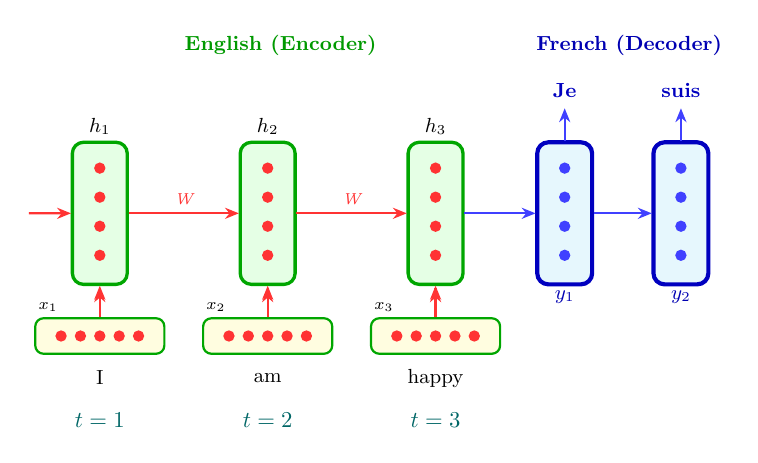
\begin{tikzpicture}[
  >=Stealth, thick,
  enc/.style={draw=green!65!black, fill=green!10, rounded corners=4pt,
              minimum width=0.85cm, minimum height=2.2cm, line width=1.2pt},
  dec/.style={draw=blue!75!black, fill=cyan!10, rounded corners=4pt,
              minimum width=0.85cm, minimum height=2.2cm, line width=1.5pt},
  emb/.style={draw=green!65!black, fill=yellow!12, rounded corners=3pt,
              minimum width=2.0cm, minimum height=0.55cm},
  rdot/.style={circle, fill=red!80, minimum size=5pt, inner sep=0pt},
  bdot/.style={circle, fill=blue!75, minimum size=5pt, inner sep=0pt},
  rarr/.style={-{Stealth[length=5pt,width=4pt]}, thick, red!80},
  barr/.style={-{Stealth[length=5pt,width=4pt]}, thick, blue!75},
  scale=0.82, transform shape
]

%% Language labels
\node[font=\small\bfseries, text=green!60!black] at (2.8,2.8)  {English (Encoder)};
\node[font=\small\bfseries, text=blue!70!black]  at (8.2,2.8)  {French (Decoder)};

%% Encoder cells
\foreach \x/\lab/\nm in {0.0/$h_1$/h1, 2.6/$h_2$/h2, 5.2/$h_3$/h3}{
  \node[enc](\nm) at (\x,0.2){};
  \foreach \y in {0.9, 0.45, 0.0, -0.45}{\node[rdot] at (\x,\y){};}
  \node[font=\small\itshape] at (\x,1.55) {\lab};
}
\draw[rarr] (-1.1,0.2) -- (h1.west);
\draw[rarr] (h1.east) -- (h2.west) node[midway,above,font=\scriptsize\itshape]{W};
\draw[rarr] (h2.east) -- (h3.west) node[midway,above,font=\scriptsize\itshape]{W};

%% Input embeddings
\foreach \xc/\lbl/\word in {0.0/$x_1$/I, 2.6/$x_2$/am, 5.2/$x_3$/happy}{
  \node[emb](xe\word) at (\xc,-1.7){};
  \foreach \dx in {-0.6,-0.3,0,0.3,0.6}{\node[rdot] at (\xc+\dx,-1.7){};}
  \node[font=\scriptsize\itshape] at (\xc-0.8,-1.25) {\lbl};
  \node[font=\small] at (\xc,-2.35) {\word};
  \draw[rarr] (xe\word.north) -- ++(0,0.45);
}
\draw[rarr] (xeI.north)++(0,0.45) -- (h1.south);
\draw[rarr] (xeam.north)++(0,0.45) -- (h2.south);
\draw[rarr] (xehappy.north)++(0,0.45) -- (h3.south);

%% Decoder cells
\node[dec](d1) at (7.2,0.2){};
\foreach \y in {0.9,0.45,0.0,-0.45}{\node[bdot] at (7.2,\y){};}
\node[dec](d2) at (9.0,0.2){};
\foreach \y in {0.9,0.45,0.0,-0.45}{\node[bdot] at (9.0,\y){};}
\node[font=\small\itshape, text=blue!70!black] at (7.2,-1.1) {$y_1$};
\node[font=\small\itshape, text=blue!70!black] at (9.0,-1.1) {$y_2$};
\node[font=\small\bfseries, text=blue!75!black] at (7.2,2.1) {Je};
\node[font=\small\bfseries, text=blue!75!black] at (9.0,2.1) {suis};
\draw[barr] (h3.east) -- ++(0.55,0) |- (d1.west);
\draw[barr] (d1.east) -- (d2.west);
\draw[barr] (d1.north) -- ++(0,0.5);
\draw[barr] (d2.north) -- ++(0,0.5);

%% Timestep annotations
\foreach \x/\t in {0.0/1, 2.6/2, 5.2/3}{
  \node[font=\normalsize\bfseries, text=teal!80!black] at (\x,-3.0) {$t=\t$};
}
\end{tikzpicture}
\caption{LSTM encoder--decoder for sequence-to-sequence translation
  (\textit{``I am happy''} $\to$ \textit{``Je suis \ldots''}). The encoder
  processes tokens sequentially, passing hidden state $h_t$ forward; the
  decoder generates the target sequence conditioned on the final encoder state.}
\label{fig:lstm}
\end{figure}

\subsection{Limitations of the LSTM}

While the LSTM addresses the vanishing gradient problem, it has three remaining
weaknesses that limit its effectiveness for language understanding:

\begin{description}[leftmargin=2em, style=nextline]
  \item[\textbf{1.~Sequential bottleneck.}]
    The recurrence $h_t = f(h_{t-1}, x_t)$ is inherently sequential: token $t$
    cannot be processed until token $t{-}1$ is complete. This prevents
    parallelisation along the time axis, making training slow on long sequences.

  \item[\textbf{2.~Memory degradation.}]
    Despite the gating mechanism, information from early tokens is progressively
    diluted over many timesteps. For a sequence of length $T$, the influence of
    $x_1$ on $h_T$ decays roughly as $\prod_{t=2}^{T} f_t$ --- a product of
    forget gate values all $\leq 1$.

  \item[\textbf{3.~Unidirectionality.}]
    A left-to-right LSTM builds the representation of token $t$ from only its
    left context $x_1, \ldots, x_{t-1}$. The right context --- which is often
    crucial for disambiguation --- is unavailable.
\end{description}

\subsection{Bidirectional LSTM (BiLSTM)}
\label{subsec:bilstm}

The \textbf{Bidirectional LSTM}~\cite{schuster1997bilstm} (BiLSTM) attempts to
address the unidirectionality problem by running two separate LSTM passes over
the input --- a forward pass (left-to-right) producing $\overrightarrow{h_t}$
and a backward pass (right-to-left) producing $\overleftarrow{h_t}$ --- and
concatenating their outputs:
\begin{equation}
  h_t = \left[\overrightarrow{h_t}\,;\,\overleftarrow{h_t}\right]
  \label{eq:bilstm}
\end{equation}

% ── BiLSTM diagram ────────────────────────────────────────────────────────────
\begin{figure}[H]
\centering
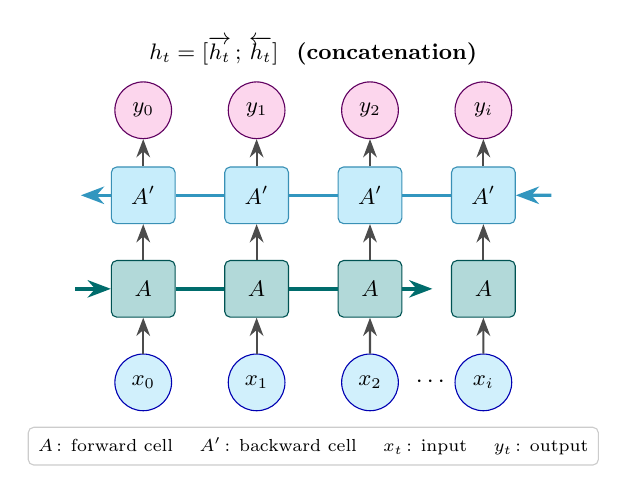
\begin{tikzpicture}[
  >=Stealth, x=1.6cm, y=1.2cm,
  xnode/.style={circle, draw=blue!70!black, fill=cyan!18,
                minimum size=8mm, inner sep=0pt, font=\small},
  ynode/.style={circle, draw=violet!75!black, fill=magenta!16,
                minimum size=8mm, inner sep=0pt, font=\small},
  fcell/.style={draw=teal!65!black, fill=teal!30, rounded corners=2pt,
                minimum width=9mm, minimum height=8mm, font=\small\bfseries},
  bcell/.style={draw=cyan!70!black, fill=cyan!22, rounded corners=2pt,
                minimum width=9mm, minimum height=8mm, font=\small\bfseries},
  fwd/.style={->, very thick, teal!85!black},
  bwd/.style={->, very thick, cyan!75!black},
  conn/.style={->, thick, black!70},
  scale=0.9, transform shape
]

\def\ymid{0} \def\ytop{1.1} \def\ybot{-1.1}

\foreach \x/\idx in {0/0,1/1,2/2,3/i}{
  \node[xnode](x\idx) at (\x,\ybot) {$x_{\idx}$};
  \node[ynode](y\idx) at (\x,\ytop+1.0) {$y_{\idx}$};
  \node[fcell](f\idx) at (\x,\ymid) {$A$};
  \node[bcell](b\idx) at (\x,\ytop) {$A'$};
  \draw[conn] (x\idx)--(f\idx);
  \draw[conn] (f\idx.north) to[out=90,in=-90] (b\idx.south);
  \draw[conn] (b\idx.north) -- (y\idx.south);
}
\node[font=\normalsize] at (2.55,\ybot) {$\cdots$};

\draw[fwd] (-0.6,\ymid) -- (f0);
\draw[fwd] (f0)--(f1) (f1)--(f2) (f2)--++(0.55,0);

\draw[bwd] (3.6,\ytop) -- (bi);
\draw[bwd] (bi)--(b2) (b2)--(b1) (b1)--(b0) (b0)--++(-0.55,0);

\node[draw=black!20, fill=white, rounded corners=2pt,
      font=\scriptsize, align=left, inner sep=4pt]
  at (1.5,-1.85)
  {$A$\,: forward cell \quad $A'$\,: backward cell \quad
   $x_t$\,: input \quad $y_t$\,: output};

\node[font=\small\bfseries] at (1.5, 2.8)
  {$h_t = [\overrightarrow{h_t}\,;\,\overleftarrow{h_t}]$ \ (concatenation)};

\end{tikzpicture}
\caption{Bidirectional LSTM (BiLSTM). A forward pass (teal, $A$) processes
  tokens left-to-right; a backward pass (cyan, $A'$) processes tokens
  right-to-left. The outputs are concatenated at each position to form a
  context-aware representation. The two passes are trained independently and
  merged only at the output.}
\label{fig:bilstm}
\end{figure}

The BiLSTM provides richer representations than a unidirectional LSTM.
ELMo~\cite{peters2018elmo} (Peters et al., 2018), a prominent pre-\bert{}
contextualised embedding model, uses a stacked BiLSTM and demonstrated that
contextualised representations transfer effectively to downstream tasks.
However, the BiLSTM still inherits two critical limitations:

\begin{itemize}[leftmargin=2em]
  \item \textbf{Not truly bidirectional.} The forward and backward passes are
        trained \emph{separately} and only combined at the output
        (Eq.~\ref{eq:bilstm}). The two directions never interact during feature
        extraction; the model cannot, within a single layer, allow left-context
        and right-context information to jointly influence each other.
  \item \textbf{Still sequential.} Both passes remain sequential along their
        respective directions, limiting parallelisation and scalability.
\end{itemize}

% =============================================================================
\section{The Transformer Architecture}
\label{sec:transformer}
% =============================================================================

\subsection{Motivation and Core Idea}

Both LSTM variants process text token by token. The root cause of their
limitations is the sequential recurrence: dependency on the previous hidden
state forces one-at-a-time computation and creates an information bottleneck for
long-range dependencies.

The \textbf{Transformer}~\cite{vaswani2017attention} (Vaswani et al., 2017)
discards recurrence entirely. Its central mechanism is \textbf{self-attention}:
every token directly attends to every other token in the sequence
\emph{simultaneously}, computing a weighted combination of all position
representations in a single operation.

\subsection{Self-Attention Mechanism}
\label{subsec:selfattn}

Given an input sequence of $n$ tokens represented as a matrix
$X \in \R^{n \times d_{\text{model}}}$, three linear projections produce query,
key, and value matrices:
\begin{equation}
  Q = X W^Q, \quad K = X W^K, \quad V = X W^V
  \label{eq:qkv}
\end{equation}
where $W^Q, W^K, W^V \in \R^{d_{\text{model}} \times d_k}$.
The \textbf{scaled dot-product attention} output is:
\begin{equation}
  \text{Attention}(Q, K, V)
    = \softmax\!\left(\frac{QK^\top}{\sqrt{d_k}}\right) V
  \label{eq:attention}
\end{equation}

The scaling factor $1/\sqrt{d_k}$ prevents the dot products from growing large
in magnitude, which would push the softmax into regions of extremely small
gradients. Each output row is a weighted sum of all value vectors, where the
weights reflect how relevant each token is to the current query position.

\subsection{Multi-Head Attention}

Rather than performing a single attention operation, the Transformer applies $h$
\emph{parallel} attention heads, each learning a different projection:
\begin{equation}
  \text{MultiHead}(Q,K,V)
    = \text{Concat}(\text{head}_1, \ldots, \text{head}_h)\, W^O
  \label{eq:multihead}
\end{equation}
where $\text{head}_i = \text{Attention}(QW_i^Q,\, KW_i^K,\, VW_i^V)$ and
$W^O \in \R^{hd_k \times d_{\text{model}}}$. Multiple heads allow the model
to capture different types of relationships simultaneously --- \textit{e.g.}\
syntactic agreement, coreference, and semantic similarity --- from the same
input.

% ── Self-attention illustration ───────────────────────────────────────────────
\begin{figure}[H]
\centering
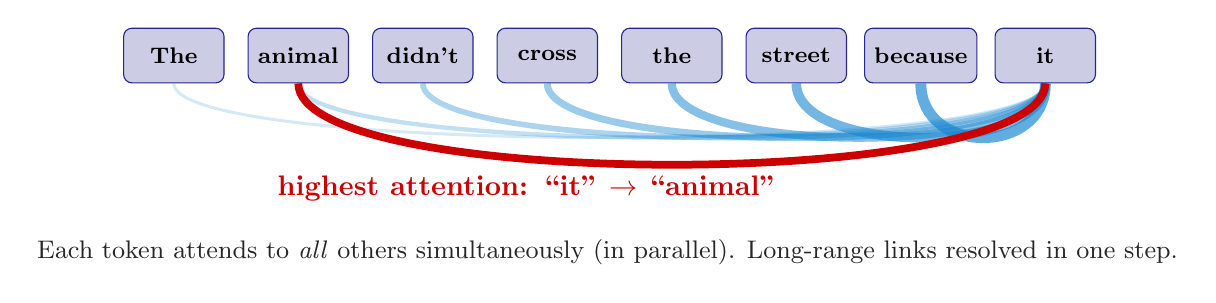
\begin{tikzpicture}[>=Stealth, scale=1.02, transform shape]
  \def\words{{"The","animal","didn't","cross","the","street","because","it"}}
  \foreach \i in {0,...,7}{
    \pgfmathsetmacro{\lbl}{\words[\i]}
    \node[draw=NavyBlue!85, fill=NavyBlue!20, rounded corners=3pt,
          minimum width=1.25cm, minimum height=0.68cm,
          font=\footnotesize\bfseries, align=center, text=black]
          (tok\i) at ({-5.4 + \i*1.55}, 0) {\lbl};
  }
  \foreach \i in {0,1,2,3,4,5,6}{
    \pgfmathsetmacro{\opac}{0.18 + \i*0.08}
    \draw[cyan!65!blue, opacity=\opac, line width={\opac*6pt}]
      (tok7.south) .. controls +(0,-0.9) and +(0,-0.9) .. (tok\i.south);
  }
  \draw[red!80!black, very thick, line width=2.8pt]
    (tok7.south) .. controls +(0,-1.35) and +(0,-1.35) .. (tok1.south);
  \node[font=\normalsize\bfseries, text=red!80!black] at (-1.0,-1.65)
    {highest attention: ``it'' $\rightarrow$ ``animal''};
  \node[font=\small, text=black!85, align=center] at (0,-2.45)
    {Each token attends to \emph{all} others simultaneously (in parallel).
     Long-range links resolved in one step.};
\end{tikzpicture}
\caption{Self-attention in action. The pronoun \textit{``it''} attends most
  strongly to \textit{``animal''}, resolving the coreference in a single layer
  without traversing a chain of timesteps. Thicker arcs indicate higher
  attention weights.}
\label{fig:selfattn}
\end{figure}

\subsection{Positional Encoding}

Since self-attention is permutation-invariant (Eq.~\ref{eq:attention} has no
notion of token order), the Transformer injects \textbf{positional
encodings}~\cite{vaswani2017attention} into the input embeddings:
\begin{equation}
  \text{PE}_{(pos,\,2i)}   = \sin\!\left(\frac{pos}{10000^{2i/d}}\right),
  \qquad
  \text{PE}_{(pos,\,2i+1)} = \cos\!\left(\frac{pos}{10000^{2i/d}}\right)
  \label{eq:posenc}
\end{equation}
These fixed sinusoidal functions encode absolute position and allow the model to
represent relative distances between tokens.

\subsection{Encoder and Decoder Stacks}

The original Transformer~\cite{vaswani2017attention} is an encoder--decoder
model. Each encoder layer consists of (i)~multi-head self-attention and
(ii)~a position-wise feed-forward network (FFN), each sublayer wrapped with a
residual connection and Layer Normalisation. The decoder additionally contains
a \emph{cross-attention} sublayer that queries the encoder output.

\begin{figure}[H]
  \centering
  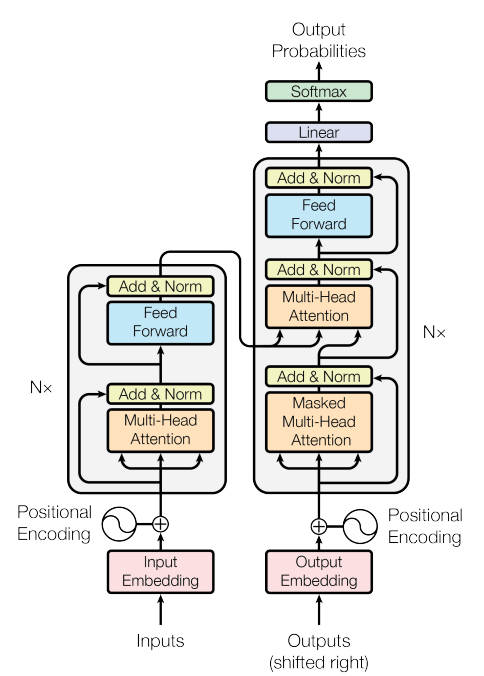
\includegraphics[width=0.75\textwidth]{og_transformer.png}
  \caption{The original Transformer architecture~\cite{vaswani2017attention}.
    The encoder (left) produces contextual embeddings from the source sequence.
    The decoder (right) generates the target sequence auto-regressively, using
    masked self-attention and cross-attention over the encoder output.}
  \label{fig:transformer}
\end{figure}

\subsection{Why the Transformer Surpasses the LSTM}

Table~\ref{tab:lstm_vs_transformer} summarises the key differences between the
two architectures.

\begin{table}[H]
\centering
\caption{LSTM vs.\ Transformer: a direct comparison.}
\label{tab:lstm_vs_transformer}
\begin{tabularx}{0.92\textwidth}{lXX}
  \toprule
  \textbf{Property} & \textbf{LSTM / BiLSTM} & \textbf{Transformer} \\
  \midrule
  Parallelism
    & Sequential; one step per token
    & Fully parallel over all tokens \\
  Long-range dependencies
    & Degrade with distance
    & Constant path length between any two positions \\
  Bidirectionality
    & Separate forward/backward passes
    & Joint left+right context within every attention layer \\
  Scalability
    & Hard to scale to very long sequences
    & Scales with hardware via parallelism \\
  \bottomrule
\end{tabularx}
\end{table}

% =============================================================================
\section{Introduction to \bert{}}
\label{sec:intro_bert}
% =============================================================================

\subsection{From Transformer to \bert{}}

The Transformer's encoder already attends bidirectionally: in each
self-attention head, every token can query every other token regardless of
direction. However, the original Transformer was designed as an encoder--decoder
for sequence-to-sequence tasks. \textbf{\bert{}}~\cite{devlin2019bert} (Devlin
et al., 2018) makes a deliberate choice: \emph{keep only the encoder stack} and
pre-train it for language understanding rather than generation.

\begin{figure}[H]
  \centering
  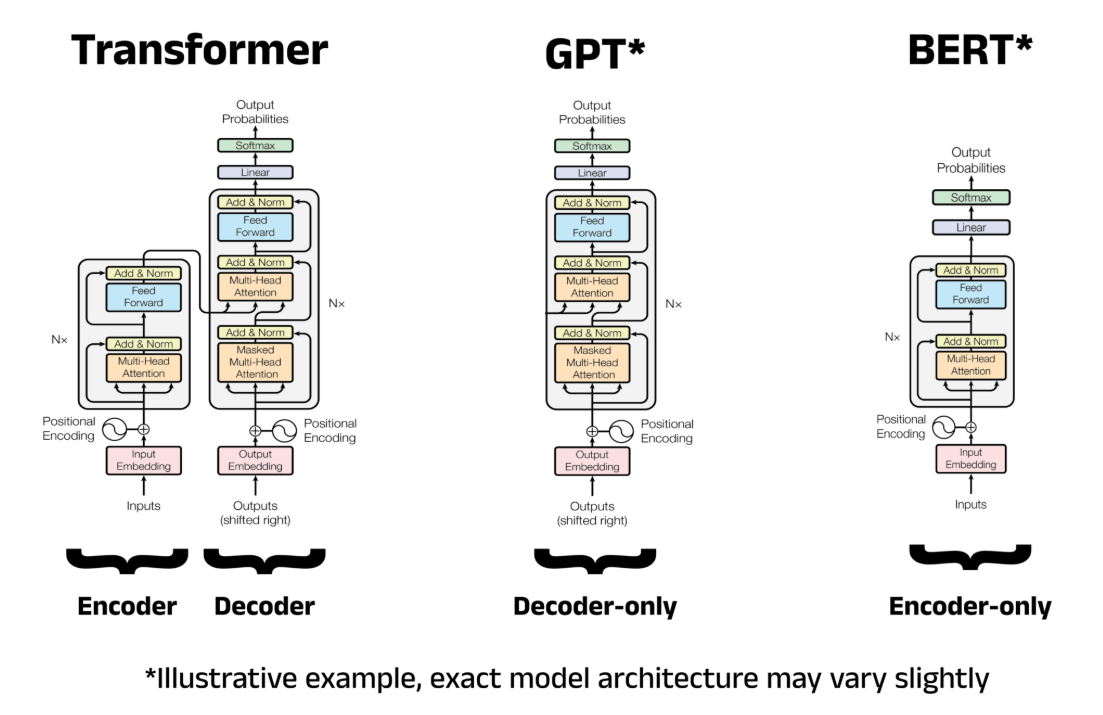
\includegraphics[width=\textwidth]{comparison.png}
  \caption{Architectural comparison. The original Transformer uses both
    encoder and decoder for translation. \bert{} retains only the encoder stack,
    using the \cls{} token representation as input to task-specific classifier
    heads.}
  \label{fig:bert_vs_transformer}
\end{figure}

Table~\ref{tab:transformer_vs_bert} contrasts the two architectures.

\begin{table}[H]
\centering
\caption{Original Transformer vs.\ \bert{}.}
\label{tab:transformer_vs_bert}
\begin{tabularx}{0.92\textwidth}{lXX}
  \toprule
  \textbf{Aspect}
    & \textbf{Original Transformer}~\cite{vaswani2017attention}
    & \textbf{\bert{}}~\cite{devlin2019bert} \\
  \midrule
  Architecture
    & Encoder + Decoder
    & Encoder only ($N$ stacked layers) \\
  Primary task
    & Sequence-to-sequence (translation)
    & Representation learning / understanding \\
  Context
    & Decoder is left-to-right (masked)
    & Fully bidirectional at every layer \\
  Pre-training
    & None (direct supervision)
    & Masked LM + Next Sentence Prediction \\
  Usage
    & Train end-to-end per task
    & Pre-train once, fine-tune per task \\
  \bottomrule
\end{tabularx}
\end{table}

\begin{remark}
  \textit{``The Transformer learns to \textbf{translate}. \bert{} learns to
  \textbf{understand}.''}
\end{remark}

\subsection{What Makes \bert{} Truly Bidirectional?}

This is a subtle but crucial point. ELMo~\cite{peters2018elmo} was also called
``bidirectional,'' but its forward and backward LSTMs were trained with separate
language model objectives and then concatenated. \bert{}, by contrast, uses a
\emph{single unified} Transformer encoder in which every attention head
simultaneously sees all tokens from both directions, and every layer integrates
left and right context jointly. This \emph{deep} bidirectionality --- as opposed
to shallow concatenation --- is what makes \bert{}'s representations
qualitatively different.
% =============================================================================
\section{Why \bert{} Was a Turning Point}
\label{sec:turning_point}
% =============================================================================

\subsection{Pre-training Objectives}

\bert{} is pre-trained on two self-supervised tasks using only unlabelled text
(Wikipedia + BookCorpus, $\approx$3.3 billion words):

\subsubsection{Masked Language Model (MLM)}

Inspired by the Cloze task~\cite{taylor1953cloze}, 15\% of input tokens are
randomly masked. \bert{} is trained to predict the original token from its
\emph{bidirectional} context:
\begin{equation}
  \mathcal{L}_{\text{MLM}}
    = -\sum_{i \in \mathcal{M}}
      \log P\!\left(x_i \mid x_1, \ldots, x_{i-1},
      \mask{}, x_{i+1}, \ldots, x_n\right)
  \label{eq:mlm}
\end{equation}
where $\mathcal{M}$ is the set of masked positions. Because a correct prediction
requires integrating context from \emph{both} sides, this objective inherently
forces the model to learn deeply bidirectional representations. Traditional
left-to-right language models cannot use this objective without a fundamental
architectural change.

\subsubsection{Next Sentence Prediction (NSP)}

Many NLP tasks (\textit{e.g.}\ question answering and natural language
inference) require understanding the \emph{relationship} between two sentences.
\bert{} is therefore also trained on a binary classification task: given a
sentence pair $(A, B)$, predict whether $B$ is the sentence that actually
follows $A$ in the corpus or a randomly sampled sentence. This trains the model
to encode inter-sentence coherence in the \cls{} token.

\subsection{Fine-tuning Paradigm}

After pre-training, \bert{}'s weights serve as a starting point for any
downstream NLP task. A lightweight task-specific head is appended:

\begin{itemize}[leftmargin=2em, itemsep=2pt]
  \item \textbf{Classification} (sentiment, topic): linear layer on the
        \cls{} representation.
  \item \textbf{Token labelling / NER}: token-level classifier on each output
        position.
  \item \textbf{Extractive QA}: two linear layers predicting span start and end
        positions.
  \item \textbf{Natural Language Inference}: classification on \cls{} for
        entailment / contradiction / neutral.
\end{itemize}

Fine-tuning requires only 2--4 epochs, making \bert{} highly data-efficient.
The same pre-trained model handles all four task types with no structural
changes to the core encoder.

\subsection{Impact: State-of-the-Art Results}

Upon release, \bert{} set new state-of-the-art results across eleven NLP
benchmarks~\cite{devlin2019bert}:

\begin{table}[H]
\centering
\caption{Selected benchmark results at the time of \bert{}'s
  release~\cite{devlin2019bert}.}
\label{tab:results}
\begin{tabular}{llll}
  \toprule
  \textbf{Benchmark} & \textbf{Task} & \textbf{Prior SOTA} & \textbf{\bert{}} \\
  \midrule
  GLUE~\cite{wang2018glue}
    & Multi-task NLU            & 72.8  & 80.4 \\
  SQuAD v1.1~\cite{rajpurkar2016squad}
    & Reading comprehension (F1) & 91.7  & 93.2 \\
  SQuAD v2.0~\cite{rajpurkar2018squad2}
    & Unanswerable QA (F1)       & 78.0  & 83.1 \\
  MultiNLI~\cite{williams2018multinli}
    & Natural language inference & 86.7  & 86.7$^{+}$ \\
  \bottomrule
\end{tabular}
\end{table}

On SQuAD v1.1, \bert{} exceeded human performance on the F1 metric. Crucially,
these results came from a \emph{single} pre-trained model fine-tuned separately
for each task, demonstrating that rich, general-purpose language representations
can be learned once and deployed everywhere.

\subsection{Why It Was a Paradigm Shift}

Four reasons make \bert{} a genuine turning point in NLP:

\begin{enumerate}[leftmargin=2em, itemsep=3pt]
  \item \textbf{Deep bidirectionality at scale.} Unlike ELMo's shallow
        concatenation of separately trained LSTMs, \bert{} integrates left and
        right context jointly in every layer, yielding fundamentally richer
        token representations.

  \item \textbf{Transfer learning for NLP.} \bert{} demonstrated that the
        ``pre-train on unlabelled data, fine-tune on small labelled data''
        paradigm --- long established in computer vision --- works powerfully for
        language. This shifted NLP research away from task-specific architectures
        towards general-purpose pre-trained models.

  \item \textbf{Open release.} Google released \bert{}'s weights, code, and
        pre-training procedure publicly, enabling rapid community adoption and
        spawning a generation of derivative models: RoBERTa~\cite{liu2019roberta},
        DistilBERT~\cite{sanh2019distilbert}, ALBERT~\cite{lan2019albert},
        domain-specific variants, and multilingual extensions.

  \item \textbf{Contextual representations by design.} Every output embedding
        depends on the full sentence context through every attention layer,
        resolving polysemy as an architectural consequence rather than an
        optional post-processing step.
\end{enumerate}


% =============================================================================
\section{High-Level Architecture Overview}
\label{sec:arch}
% =============================================================================

This section briefly describes \bert{}'s architecture. Detailed analysis of each
component will be covered in the subsequent team sections.

\subsection{Input Representation}

\bert{} constructs each input token's embedding as the sum of three learned
components~\cite{devlin2019bert}:
\begin{equation}
  E_{\text{input}}
    = E_{\text{token}} + E_{\text{segment}} + E_{\text{position}}
  \label{eq:input}
\end{equation}
where $E_{\text{token}}$ is a WordPiece~\cite{wu2016wordpiece} subword embedding
($|V| \approx 30{,}000$), $E_{\text{segment}}$ distinguishes sentence~$A$ from
sentence~$B$ in a paired input, and $E_{\text{position}}$ is a learned
positional embedding. A special \cls{} token is prepended to every input;
\sep{} marks sentence boundaries.

\subsection{Encoder Stack}

\bert{} stacks $N$ identical Transformer encoder layers
(Section~\ref{sec:transformer}). Each layer applies multi-head self-attention
(Eq.~\ref{eq:multihead}), Add \& Norm, a feed-forward sublayer, and another
Add \& Norm. Two standard configurations were released:

\begin{table}[H]
\centering
\caption{\bert{} model variants~\cite{devlin2019bert}.}
\label{tab:bert_variants}
\begin{tabular}{lcccc}
  \toprule
  \textbf{Variant}
    & \textbf{Layers ($N$)}
    & \textbf{Hidden size ($d$)}
    & \textbf{Heads ($h$)}
    & \textbf{Parameters} \\
  \midrule
  \bert{}\textsubscript{BASE}  & 12 & 768  & 12 & $\approx$110M \\
  \bert{}\textsubscript{LARGE} & 24 & 1024 & 16 & $\approx$340M \\
  \bottomrule
\end{tabular}
\end{table}

\noindent
The output of the final encoder layer provides one contextual embedding per
input token. These embeddings are consumed by the task-specific heads described
in Section~\ref{sec:turning_point}.
% ============================================================
%  Section 2: BERT Architecture
% ============================================================

\section{BERT Architecture}
\label{sec:architecture}

\bert{} is built exclusively upon the \emph{encoder} stack of the original
Transformer architecture proposed by Vaswani~et~al.~\cite{vaswani2017attention}.
Unlike the full encoder-decoder Transformer used for sequence-to-sequence tasks,
\bert{} discards the decoder entirely; its objective is to produce rich contextual
representations of input tokens rather than to autoregressively generate output
sequences.

\subsection{Transformer Encoder Stack}
\label{subsec:encoder}

The model consists of $L$ identical encoder layers stacked sequentially.  Each
layer $\ell \in \{1, \ldots, L\}$ transforms its input representation
$\mathbf{H}^{(\ell-1)} \in \R^{n \times d}$ (where $n$ is the sequence length and
$d$ is the hidden dimension) into a refined output $\mathbf{H}^{(\ell)}$ through
two principal sub-layers:

\begin{enumerate}
  \item \textbf{Multi-Head Self-Attention~(MHSA).}  Tokens attend to all other
        tokens in the sequence, producing context-enriched representations.
        (Described in detail in \cref{sec:attention}.)

  \item \textbf{Position-Wise Feed-Forward Network~(FFN).}  A pair of linear
        transformations with a $\gelu$ non-linearity is applied independently to
        each token position.
\end{enumerate}

\noindent Both sub-layers are wrapped with \emph{residual connections} and
\emph{layer normalisation}~\cite{ba2016layer}, following the formulation:
\begin{equation}
  \mathbf{H}^{(\ell)} = \operatorname{LayerNorm}\!\bigl(
    \mathbf{z} + \operatorname{SubLayer}(\mathbf{z})
  \bigr), \quad \mathbf{z} = \mathbf{H}^{(\ell-1)}.
  \label{eq:residual}
\end{equation}
Residual connections mitigate the vanishing-gradient problem and stabilise training
in deep networks, while layer normalisation normalises activations across the hidden
dimension for each token independently.

\begin{table}[H]
  \centering
  \caption{Computation flow within a single Transformer encoder layer.  MHSA denotes
           Multi-Head Self-Attention; FFN denotes Position-Wise Feed-Forward Network.}
  \label{tab:layer_composition}
  \renewcommand{\arraystretch}{1.4}
  \begin{tabular}{lcc}
    \toprule
    \textbf{Sub-layer} & \textbf{Input} & \textbf{Output Dimension} \\
    \midrule
    MHSA  & $\mathbf{H}^{(\ell-1)} \in \mathbb{R}^{n \times d}$ & $\mathbb{R}^{n \times d}$ \\
    \hspace{0.5cm} + LayerNorm + Residual & & \\
    FFN   & $\mathbf{H}^{(\ell)} \in \mathbb{R}^{n \times d}$ & $\mathbb{R}^{n \times d}$ \\
    \hspace{0.5cm} + LayerNorm + Residual & & \\
    \bottomrule
  \end{tabular}
\end{table}

\begin{figure}[H]
  \centering
  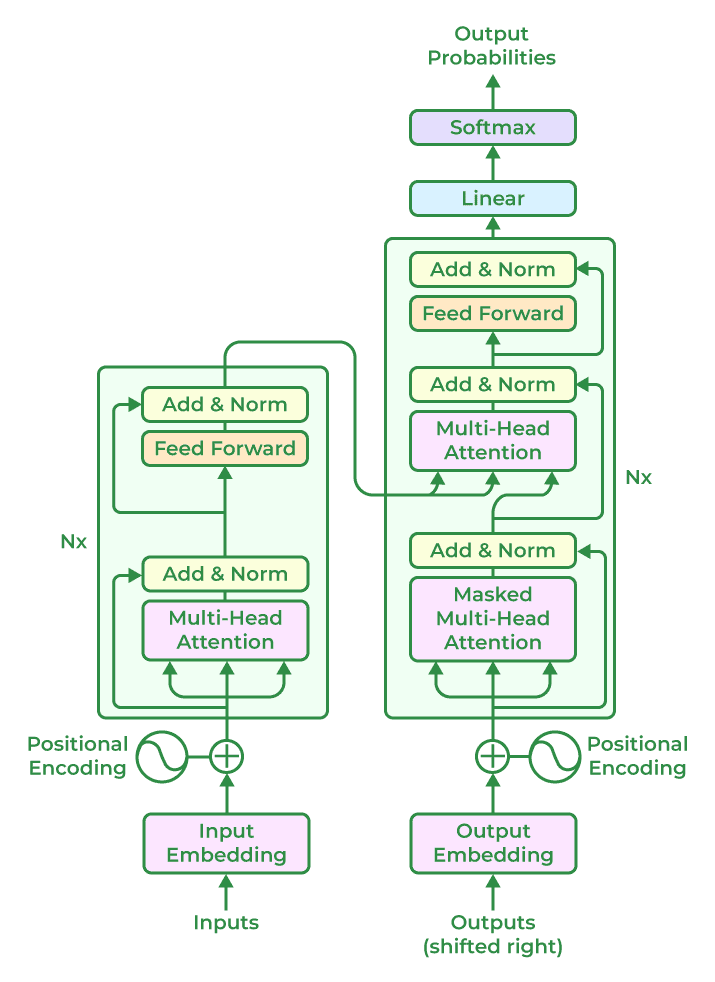
\includegraphics[width=0.72\textwidth]{figures/transformer.png}
  \caption{Stacked Transformer encoder architecture underlying \bert{}.  Each of the
           $L$ encoder layers applies Multi-Head Attention followed by a Feed-Forward
           Network, with residual connections and layer normalisation at each
           sub-layer.}
  \label{fig:transformer}
\end{figure}

\subsection{Hierarchical Representation Learning}
\label{subsec:hierarchical}

A salient property of deep Transformer encoders is their ability to construct
\emph{hierarchical} representations across layers.

\begin{itemize}
  \item \textbf{Lower layers} ($\ell \approx 1$--$4$) tend to encode surface-level
        and syntactic information such as part-of-speech tags, morphology, and
        local phrase structure~\cite{tenney2019bert}.

  \item \textbf{Middle layers} ($\ell \approx 5$--$8$) capture syntactic
        dependencies including subject-verb agreement and coreference.

  \item \textbf{Upper layers} ($\ell \approx 9$--$12$ for \bert{}-Base) encode
        high-level semantic information and task-relevant abstractions, making them
        particularly well-suited as features for downstream tasks.
\end{itemize}

This layered abstraction mirrors the hierarchical feature extraction observed in
convolutional neural networks applied to vision tasks, and it affords \bert{} the
ability to generalise across a broad range of linguistic phenomena.

\subsection{Model Configurations}
\label{subsec:configs}

Two standard configurations of \bert{} were released, differing in depth and width:

\begin{table}[H]
  \centering
  \caption{Standard \bert{} model configurations.  $L$: number of encoder layers;
           $H$: hidden dimension; $A$: number of attention heads;
           $P$: total parameter count.}
  \label{tab:configs}
  \renewcommand{\arraystretch}{1.25}
  \begin{tabular}{lcccc}
    \toprule
    \textbf{Variant} & $L$ & $H$ & $A$ & $P$ \\
    \midrule
    \bert{}-Base  & 12 & 768  & 12 & $\approx$110M \\
    \bert{}-Large & 24 & 1024 & 16 & $\approx$340M \\
    \bottomrule
  \end{tabular}
\end{table}

\bert{}-Large achieves higher performance on most benchmarks but demands
substantially greater computational resources for both pre-training and fine-tuning.
\bert{}-Base remains the standard choice for resource-constrained settings.

% ============================================================
%  Section 3: Self-Attention Mechanism
% ============================================================

\section{Self-Attention Mechanism}
\label{sec:attention}

Self-attention is the computational core of \bert{} and the mechanism that enables
every token to directly interact with every other token, regardless of their positional
distance.  Unlike recurrent architectures that process sequences step-by-step, the
self-attention operation is executed in a \emph{single parallelisable pass}, making it
both expressive and computationally efficient on modern hardware.

\subsection{Conceptual Overview}
\label{subsec:attn_concept}

At an intuitive level, self-attention allows the model to ask, for each token
position: \emph{``Given what I am looking for (query), which other tokens in the
sequence (keys) hold the information (values) I should incorporate into my updated
representation?''}  The answer is a \emph{weighted sum} of value vectors, where
the weights reflect the semantic relevance between queries and keys.

This formulation confers three key properties:

\begin{itemize}
  \item \textbf{Global receptive field.}  A token at position $i$ can directly
        attend to a token at position $j$ with $O(1)$ operations, bypassing the
        $O(n)$ path length required by RNNs.

  \item \textbf{Dynamic, content-based weighting.}  Attention weights are computed
        on-the-fly from the current input representations rather than fixed by
        positional priors.

  \item \textbf{Parallelism.}  All attention weights across all positions can be
        computed simultaneously, enabling efficient GPU/TPU utilisation.
\end{itemize}

\subsection{Mathematical Formulation}
\label{subsec:attn_math}

Given an input matrix $\mathbf{X} \in \R^{n \times d}$, three projection matrices
$\mathbf{W}^Q, \mathbf{W}^K \in \R^{d \times d_k}$ and
$\mathbf{W}^V \in \R^{d \times d_v}$ are used to produce:
\begin{equation}
  \mathbf{Q} = \mathbf{X}\mathbf{W}^Q, \quad
  \mathbf{K} = \mathbf{X}\mathbf{W}^K, \quad
  \mathbf{V} = \mathbf{X}\mathbf{W}^V.
  \label{eq:qkv}
\end{equation}
The \emph{scaled dot-product attention} is then:
\begin{equation}
  \operatorname{Attention}(\mathbf{Q}, \mathbf{K}, \mathbf{V})
  = \softmax\!\left(\frac{\mathbf{Q}\mathbf{K}^\top}{\sqrt{d_k}}\right)\mathbf{V},
  \label{eq:attention}
\end{equation}
where the scaling factor $1/\sqrt{d_k}$ prevents the dot products from growing
large in magnitude, which would push the softmax into regions of extremely small
gradients~\cite{vaswani2017attention}.

\begin{remark}
  The raw score matrix $\mathbf{Q}\mathbf{K}^\top \in \R^{n \times n}$ contains one
  scalar score $e_{ij} = \mathbf{q}_i \cdot \mathbf{k}_j$ for every ordered token
  pair $(i, j)$.  Row-wise softmax converts these into a valid probability
  distribution; the output for position $i$ is thus a convex combination of all
  value vectors, weighted by relevance to position $i$.
\end{remark}

\begin{figure}[H]
  \centering
  \begin{minipage}[b]{0.40\textwidth}
    \centering
    \setlength{\fboxrule}{0.8pt}
    \setlength{\fboxsep}{9pt}
    \fbox{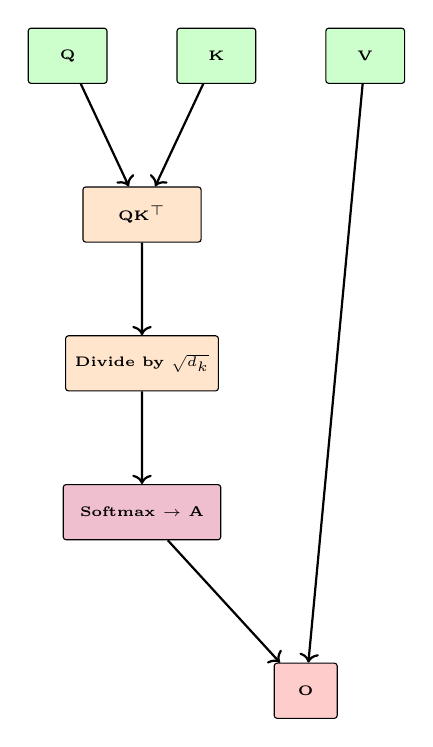
\begin{tikzpicture}[scale=1.26,
        node distance=1.5cm,
        input/.style={draw, fill=green!20, minimum width=1.0cm, minimum height=0.7cm, align=center, font=\tiny\bfseries, rounded corners=1pt},
        op/.style={draw, fill=orange!20, minimum width=1.5cm, minimum height=0.7cm, align=center, font=\tiny\bfseries, rounded corners=1pt},
        attn/.style={draw, fill=purple!25, minimum width=2.0cm, minimum height=0.7cm, align=center, font=\tiny\bfseries, rounded corners=1pt},
        output/.style={draw, fill=red!20, minimum width=0.8cm, minimum height=0.7cm, align=center, font=\tiny\bfseries, rounded corners=1pt}
      ]
      
      % Input layer
      \node[input] (Q) at (0, 4.5) {$\mathbf{Q}$};
      \node[input] (K) at (1.5, 4.5) {$\mathbf{K}$};
      \node[input] (V) at (3.0, 4.5) {$\mathbf{V}$};
      
      % Compute scores
      \node[op] (scores) at (0.75, 2.9) {$\mathbf{Q}\mathbf{K}^\top$};
      \draw[->, line width=0.8pt] (Q) -- (scores);
      \draw[->, line width=0.8pt] (K) -- (scores);
      
      % Scale
      \node[op] (scale) at (0.75, 1.4) {Divide by $\sqrt{d_k}$};
      \draw[->, line width=0.8pt] (scores) -- (scale);
      
      % Softmax → Attention weights
      \node[attn] (attn) at (0.75, -0.1) {Softmax $\to$ $\mathbf{A}$};
      \draw[->, line width=0.8pt] (scale) -- (attn);
      
      % Multiply by V and output
      \node[output] (output) at (2.4, -1.9) {$\mathbf{O}$};
      \draw[->, line width=0.8pt] (attn) -- (output);
      \draw[->, line width=0.8pt] (V) -- (output);
      
    \end{tikzpicture}}
    \subcaption{Scaled Dot-Product Attention}
    \label{fig:sdpa}
  \end{minipage}
  \hfill
  \begin{minipage}[b]{0.58\textwidth}
    \centering
    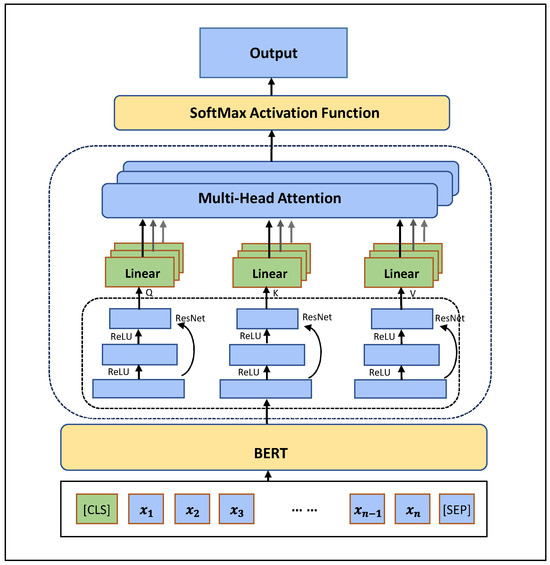
\includegraphics[width=\textwidth]{figures/multiheadattention.jpg}
    \subcaption{Multi-Head Attention}
    \label{fig:mha}
  \end{minipage}
  \caption{Attention mechanisms in BERT. (Left) Scaled dot-product attention computes relevance scores from queries and keys, applies softmax normalization to obtain attention weights $\mathbf{A}$, then aggregates values. (Right) Multi-head attention applies $h$ parallel scaled dot-product functions in projected subspaces.}
  \label{fig:attention_mechanisms}
\end{figure}

\subsection{Interpretation of Query, Key, and Value Roles}
\label{subsec:attn_roles}

\begin{itemize}
  \item \textbf{Queries} encode what a given token is \emph{seeking} from the rest
        of the sequence.
  \item \textbf{Keys} encode what information each token \emph{offers} to other
        positions.
  \item \textbf{Values} carry the actual \emph{content} to be aggregated into the
        output representation.
\end{itemize}

\noindent This abstraction is inspired by retrieval systems in information theory and
provides a powerful inductive bias for relational reasoning over sequences.

\subsection{Multi-Head Attention}
\label{subsec:multihead}

Rather than computing a single attention function, \bert{} employs $A$ parallel
\emph{attention heads}, each operating in a lower-dimensional subspace
$d_k = d_v = d/A$:
\begin{equation}
  \operatorname{head}_a = \operatorname{Attention}(
    \mathbf{Q}\mathbf{W}_a^Q,\;
    \mathbf{K}\mathbf{W}_a^K,\;
    \mathbf{V}\mathbf{W}_a^V
  ), \quad a = 1, \ldots, A.
  \label{eq:head}
\end{equation}

\begin{table}[H]
  \centering
  \caption{Attention head configuration for standard \bert{} models.  Each head
           operates independently in a projected subspace before concatenation.}
  \label{tab:attention_heads}
  \renewcommand{\arraystretch}{1.3}
  \begin{tabular}{lccccc}
    \toprule
    \textbf{Model} & $d$ & $A$ & $d_k$ & $d_v$ & Params/Head \\
    \midrule
    \bert{}-Base  & 768  & 12 & 64  & 64  & $\approx$49K \\
    \bert{}-Large & 1024 & 16 & 64  & 64  & $\approx$65K \\
    \bottomrule
  \end{tabular}
\end{table}
The outputs of all heads are concatenated and projected back to dimension $d$:
\begin{equation}
  \operatorname{MHSA}(\mathbf{Q}, \mathbf{K}, \mathbf{V})
  = \bigl[\operatorname{head}_1 \;\|\; \cdots \;\|\; \operatorname{head}_A\bigr]
    \mathbf{W}^O,
  \label{eq:multihead}
\end{equation}
where $\mathbf{W}^O \in \R^{d \times d}$ is an output projection matrix.  Multiple
heads allow the model to simultaneously attend to information from different
representational subspaces --- e.g., one head may specialise in syntactic
subject–verb relations while another focuses on coreference.

\subsection{Position-Wise Feed-Forward Network}
\label{subsec:ffn}

Following the multi-head attention sub-layer, each encoder layer applies an
identical two-layer feed-forward network independently to each token position:
\begin{equation}
  \operatorname{FFN}(\mathbf{x})
  = \gelu(\mathbf{x}\mathbf{W}_1 + \mathbf{b}_1)\mathbf{W}_2 + \mathbf{b}_2,
  \label{eq:ffn}
\end{equation}
where $\mathbf{W}_1 \in \R^{d \times d_{\mathrm{ff}}}$,
$\mathbf{W}_2 \in \R^{d_{\mathrm{ff}} \times d}$, and the inner dimension is
$d_{\mathrm{ff}} = 4d$ (e.g., 3072 for \bert{}-Base).  The $\gelu$ activation
function~\cite{hendrycks2016gelu} is a smooth approximation to ReLU that has been
found to perform better empirically in deep Transformers.

% ============================================================
%  Section 4: Input Representation
% ============================================================

\section{Input Representation}
\label{sec:input}

\bert{} does not operate on raw text but on a structured token sequence derived
through a combination of three additive embedding types.  This design allows a
single model to handle both single-sentence and sentence-pair inputs without any
architectural modification.

\subsection{Tokenisation}
\label{subsec:tokenisation}

Input text is first tokenised using \emph{WordPiece}~\cite{wu2016googles}, a
subword segmentation algorithm that decomposes rare or unseen words into frequent
sub-units drawn from a fixed vocabulary of 30,000 tokens.  For example, the word
\texttt{playing} may be split into \texttt{play} and \texttt{\#\#ing}, where the
prefix \texttt{\#\#} denotes a continuation piece.  This strategy balances
vocabulary coverage against embedding table size and reduces the out-of-vocabulary
rate to zero.

\begin{table}[H]
  \centering
  \caption{WordPiece tokenisation examples. Rare and out-of-vocabulary words are
           decomposed into frequent subword units.}
  \label{tab:tokenisation}
  \renewcommand{\arraystretch}{1.4}
  \begin{tabular}{ll}
    \toprule
    \textbf{Original Word} & \textbf{WordPiece Tokens} \\
    \midrule
    playing & [\texttt{play}, \texttt{\#\#ing}] \\
    unbelievable & [\texttt{un}, \texttt{\#\#believ}, \texttt{\#\#able}] \\
    transformer & [\texttt{transform}, \texttt{\#\#er}] \\
    \#\#ing & [\texttt{\#\#ing}] (subword only) \\
    \bottomrule
  \end{tabular}
\end{table}

\subsection{Embedding Components}
\label{subsec:embeddings}

Let $n$ denote the sequence length.  Each input position $i \in \{1, \ldots, n\}$
is associated with three embedding vectors, all of dimension $d$:

\begin{enumerate}
  \item \textbf{Token embeddings} $\mathbf{e}^{\text{tok}}_i$: a learned lookup
        table that maps each WordPiece token to a dense vector in $\R^d$.

  \item \textbf{Segment embeddings} $\mathbf{e}^{\text{seg}}_i$: one of two
        learned vectors ($\mathbf{E}_A$ or $\mathbf{E}_B$) indicating whether the
        token belongs to the first or second sentence in a sentence-pair input.
        For single-sentence inputs, all tokens receive $\mathbf{E}_A$.

  \item \textbf{Position embeddings} $\mathbf{e}^{\text{pos}}_i$: learned
        vectors for each absolute position $i \in \{0, \ldots, 511\}$, enabling
        the model to encode word order.  Note that these are \emph{learned} rather
        than the sinusoidal encodings used in the original Transformer.
\end{enumerate}

The final input representation for position $i$ is the element-wise sum:
\begin{equation}
  \mathbf{h}^{(0)}_i = \mathbf{e}^{\text{tok}}_i
    + \mathbf{e}^{\text{seg}}_i
    + \mathbf{e}^{\text{pos}}_i,
  \label{eq:embedding}
\end{equation}
and the resulting matrix $\mathbf{H}^{(0)} \in \R^{n \times d}$ is passed as
input to the first encoder layer.

\begin{figure}[H]
  \centering
  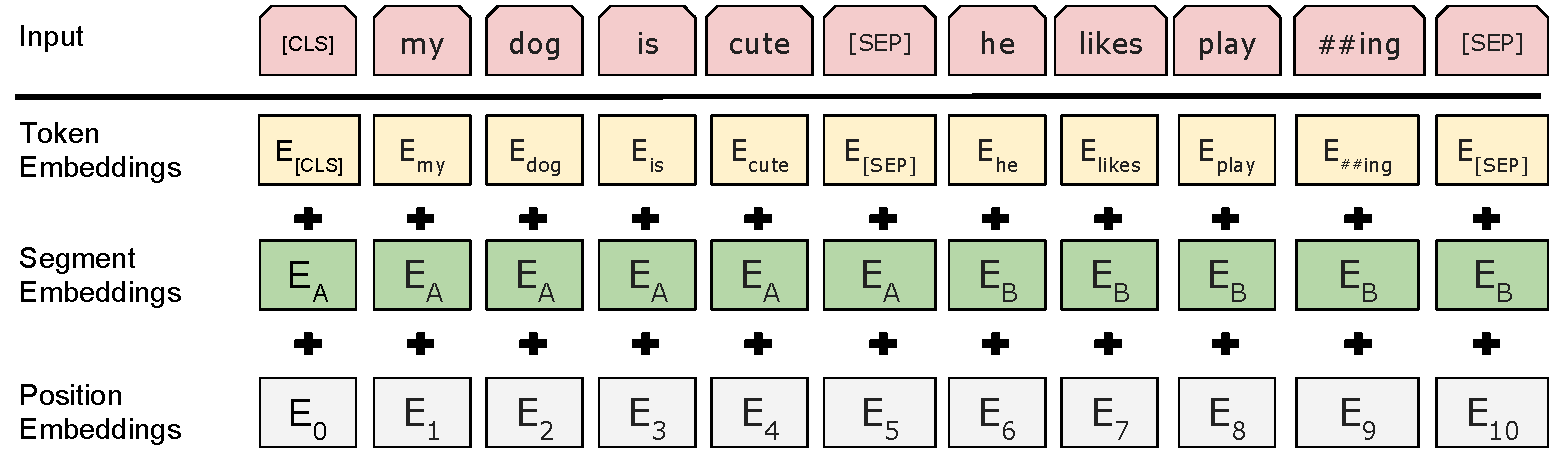
\includegraphics[width=0.90\textwidth]{figures/bert_input.pdf}
  \caption{\bert{} input representation for a sentence pair.  Each token embedding
           is summed with the corresponding segment embedding and position embedding.
           The special \cls{} token is prepended and \sep{} tokens delimit sentences.}
  \label{fig:bert_input}
\end{figure}

\subsection{Special Tokens}
\label{subsec:special_tokens}

\bert{} introduces two special tokens that carry structural significance:

\begin{itemize}
  \item \cls{} (\emph{classification token}): prepended to every input sequence.
        After passing through all $L$ encoder layers, the final hidden state
        corresponding to \cls{} aggregates a sentence-level (or sentence-pair-level)
        representation and is used as input to classification heads during
        fine-tuning.

  \item \sep{} (\emph{separator token}): inserted at the end of each sentence in a
        pair to provide an explicit boundary signal.  For single-sentence inputs, a
        single \sep{} is appended at the end.
\end{itemize}

\begin{remark}
  The maximum input length supported by BERT is 512 tokens (determined by the
  range of its learned position embeddings).  For documents exceeding this limit,
  truncation or sliding-window strategies must be employed.
\end{remark}

% ============================================================
%  Section 5: Pre-training Strategy
% ============================================================

\section{Pre-training Strategy}
\label{sec:pretraining}

\bert{} is pre-trained via \emph{self-supervised learning} on large unlabelled
corpora.  Two complementary objectives are optimised jointly, allowing the model to
acquire both token-level and sentence-level linguistic understanding.

\subsection{Masked Language Modelling (MLM)}
\label{subsec:mlm}

The MLM objective is the principal innovation that distinguishes \bert{} from
left-to-right pre-training approaches.

\paragraph{Procedure.}  At each training step, $15\%$ of the WordPiece tokens in
an input sequence are selected uniformly at random.  Of these selected tokens:
\begin{itemize}
  \item $80\%$ are replaced by the special \mask{} token;
  \item $10\%$ are replaced by a randomly sampled vocabulary token; and
  \item $10\%$ are left unchanged.
\end{itemize}
The model is then trained to predict the \emph{original} token at each masked
position using its final hidden state, producing the probability:
\begin{equation}
  P\!\left(w_i \mid \mathbf{x}_{\setminus i}\right)
  = \softmax\!\left(\mathbf{W}_o\,\mathbf{h}_i^{(L)} + \mathbf{b}_o\right),
  \label{eq:mlm}
\end{equation}
where $\mathbf{h}_i^{(L)}$ is the top-layer hidden state for position $i$,
$\mathbf{W}_o \in \R^{|\mathcal{V}| \times d}$ is a learned output projection, and
$|\mathcal{V}|$ is the vocabulary size.

\paragraph{Significance.}  Because the hidden state for a masked token is computed
from its \emph{full bilateral context}, the model is forced to integrate information
from both directions simultaneously.  This is fundamentally different from
autoregressive LMs, where causally masked attention prevents right-to-left
information flow.

\paragraph{Training signal quality.}  The 10\% random replacement and 10\%
unchanged strategies are crucial: they prevent the model from learning that
\mask{} always indicates a position to predict, while still providing the majority
of gradient signal through masked positions.

\begin{table}[H]
  \centering
  \caption{Masked Language Modelling (MLM) token treatment strategy. For each of
           the 15\% selected tokens, the replacement is chosen probabilistically.}
  \label{tab:mlm_strategy}
  \renewcommand{\arraystretch}{1.4}
  \begin{tabular}{lcc}
    \toprule
    \textbf{Action} & \textbf{Proportion} & \textbf{Purpose} \\
    \midrule
    Replace with [MASK] & $80\%$ & Primary training signal \\
    Replace with random token & $10\%$ & Encoder robustness \\
    Keep unchanged & $10\%$ & Prevent [MASK] recognition \\
    \bottomrule
  \end{tabular}
\end{table}

\subsection{Next Sentence Prediction (NSP)}
\label{subsec:nsp}

Many downstream tasks --- notably natural language inference, question answering,
and reading comprehension --- require the model to reason about relationships
\emph{between} sentences.  To pre-train this capability, \bert{} introduces an
auxiliary binary classification task.

\paragraph{Construction.}  For each training example, a sentence pair~$(A, B)$ is
constructed as follows:
\begin{itemize}
  \item With probability $50\%$: $B$ is the sentence that actually follows $A$ in
        the source corpus (\texttt{IsNext}).
  \item With probability $50\%$: $B$ is a sentence sampled uniformly at random
        from the corpus (\texttt{NotNext}).
\end{itemize}
The final hidden state of the \cls{} token is fed into a binary classifier to
predict whether the pair is contiguous.

\paragraph{Limitations.}  Subsequent work~\cite{liu2019roberta} demonstrated that
the NSP objective provides limited benefit and can even hurt performance when the
training data is already richly informative.  RoBERTa, a later variant, omits NSP
entirely without degradation.

\subsection{Pre-training Corpora}
\label{subsec:data}

\bert{} is pre-trained on two large English corpora:
\begin{itemize}
  \item \textbf{BooksCorpus}~\cite{zhu2015aligning}: approximately 800M words of
        unpublished books, providing long contiguous passages essential for learning
        inter-sentence relations.
  \item \textbf{English Wikipedia}: approximately 2,500M words (text only;
        lists, tables, and headers excluded), providing factual and encyclopaedic
        knowledge.
\end{itemize}
In total, pre-training uses roughly 3.3B tokens and requires training for
$1\,000\,000$ steps with a batch size of 256 sequences, amounting to approximately
$4$ days on $64$ Cloud TPU v3 chips for \bert{}-Base.

\subsection{Key Observations}
\label{subsec:pretrain_obs}

\begin{enumerate}
  \item \textbf{Implicit linguistic supervision.}  No hand-labelled data is used;
        supervision is derived entirely from the structure of natural language text.
  \item \textbf{Bidirectionality.}  The MLM objective produces representations
        that encode context from both directions, unlike GPT-style left-to-right
        pre-training.
  \item \textbf{High transferability.}  The resulting representations generalise
        across tasks with orthogonal linguistic requirements, requiring only a
        small task-specific fine-tuning head.
\end{enumerate}

% ============================================================
%  Section 6: Fine-Tuning
% ============================================================

\section{Fine-Tuning}
\label{sec:finetuning}

Fine-tuning adapts the pre-trained \bert{} model to a specific downstream task by
appending a lightweight task-specific head and training \emph{all} parameters
end-to-end on labelled task data.  This stands in contrast to \emph{feature-based}
approaches (e.g., ELMo) that freeze the pre-trained encoder and use its
representations as static features.

\subsection{General Procedure}
\label{subsec:ft_procedure}

Fine-tuning proceeds as follows:
\begin{enumerate}
  \item Initialise the model with the pre-trained \bert{} weights.
  \item Construct the task-appropriate input format, inserting \cls{} and \sep{}
        tokens as required.
  \item Append a task-specific output head (typically one or two linear layers)
        on top of the relevant \bert{} output representation.
  \item Train the full model (encoder + head) jointly on the labelled training set
        using a small learning rate (typically $2\text{--}5 \times 10^{-5}$) for a
        small number of epochs (typically 3--5).
\end{enumerate}

The key advantages of this approach are its simplicity and its modest data
requirements: even with a few thousand labelled examples, fine-tuned \bert{} often
surpasses task-specific architectures trained on orders of magnitude more data.

\subsection{Task Formulations}
\label{subsec:ft_tasks}

\subsubsection{Single-Sentence Classification}
\label{ssubsec:cls}

Tasks such as sentiment analysis (SST-2) and linguistic acceptability
(CoLA)~\cite{wang2018glue} use a single sentence as input.  The final hidden state
of \cls{} is passed to a linear classifier:
\begin{equation}
  \hat{y} = \softmax(\mathbf{W}_c\,\mathbf{h}_{\cls}^{(L)} + \mathbf{b}_c),
  \label{eq:cls}
\end{equation}
where $\mathbf{W}_c \in \R^{|\mathcal{Y}| \times d}$ and $\mathcal{Y}$ is the
label set.

\subsubsection{Sentence-Pair Classification}
\label{ssubsec:pair_cls}

Tasks such as Natural Language Inference (MNLI), paraphrase detection (MRPC), and
semantic similarity (STS-B) receive a sentence pair~$(A, B)$ formatted as:
\[
  \texttt{[CLS]}\ A\ \texttt{[SEP]}\ B\ \texttt{[SEP]}.
\]
The \cls{} representation aggregates cross-sentence information through
bidirectional attention and is classified as above.

\subsubsection{Question Answering (Extractive)}
\label{ssubsec:qa}

For extractive QA tasks such as SQuAD~v1.1~\cite{rajpurkar2016squad}, the
question and passage are concatenated as the sentence pair, and the model predicts
a contiguous \emph{answer span} $(s, e)$ within the passage.  Two learned vectors
$\mathbf{w}_s, \mathbf{w}_e \in \R^d$ compute start and end logits over all
passage tokens:
\begin{equation}
  P_s(i) = \frac{\exp(\mathbf{w}_s^\top \mathbf{h}_i^{(L)})}
                 {\sum_j \exp(\mathbf{w}_s^\top \mathbf{h}_j^{(L)})}, \quad
  P_e(i) = \frac{\exp(\mathbf{w}_e^\top \mathbf{h}_i^{(L)})}
                 {\sum_j \exp(\mathbf{w}_e^\top \mathbf{h}_j^{(L)})}.
  \label{eq:qa}
\end{equation}
The predicted span is $\arg\max_{s \leq e}\, P_s(s) \cdot P_e(e)$.

\subsubsection{Named Entity Recognition (NER)}
\label{ssubsec:ner}

For sequence labelling tasks (e.g., CoNLL-2003 NER), a linear classification
layer is applied to \emph{every} token's final hidden state independently, yielding
per-token label probabilities.  The \cls{} and \sep{} tokens are excluded from the
loss computation.

\begin{table}[H]
  \centering
  \caption{\bert{} fine-tuning results on representative NLU benchmarks.  GLUE is
           a composite score; others report default metrics (Acc = accuracy,
           F1 = harmonic mean).}
  \label{tab:finetuning_results}
  \renewcommand{\arraystretch}{1.35}
  \begin{tabular}{lcccc}
    \toprule
    \textbf{Task} & \textbf{Type} & \textbf{Train Size} & \textbf{Metric} & \textbf{BERT-Base} \\
    \midrule
    MNLI & Sentence-pair (3-way) & 393K & Acc & 84.6\% \\
    QQP & Paraphrase detection & 364K & Acc/F1 & 91.3\%/88.2\% \\
    MRPC & Paraphrase & 3.7K & Acc/F1 & 89.3\%/85.4\% \\
    SST-2 & Sentiment (2-way) & 67K & Acc & 93.2\% \\
    SQuAD v1.1 & Extractive QA & 88K & F1/EM & 88.5\%/80.8\% \\
    CoNLL-2003 & NER (token-level) & 15K sent & F1 & 96.4\% \\
    \bottomrule
  \end{tabular}
\end{table}

\begin{figure}[H]
  \centering
  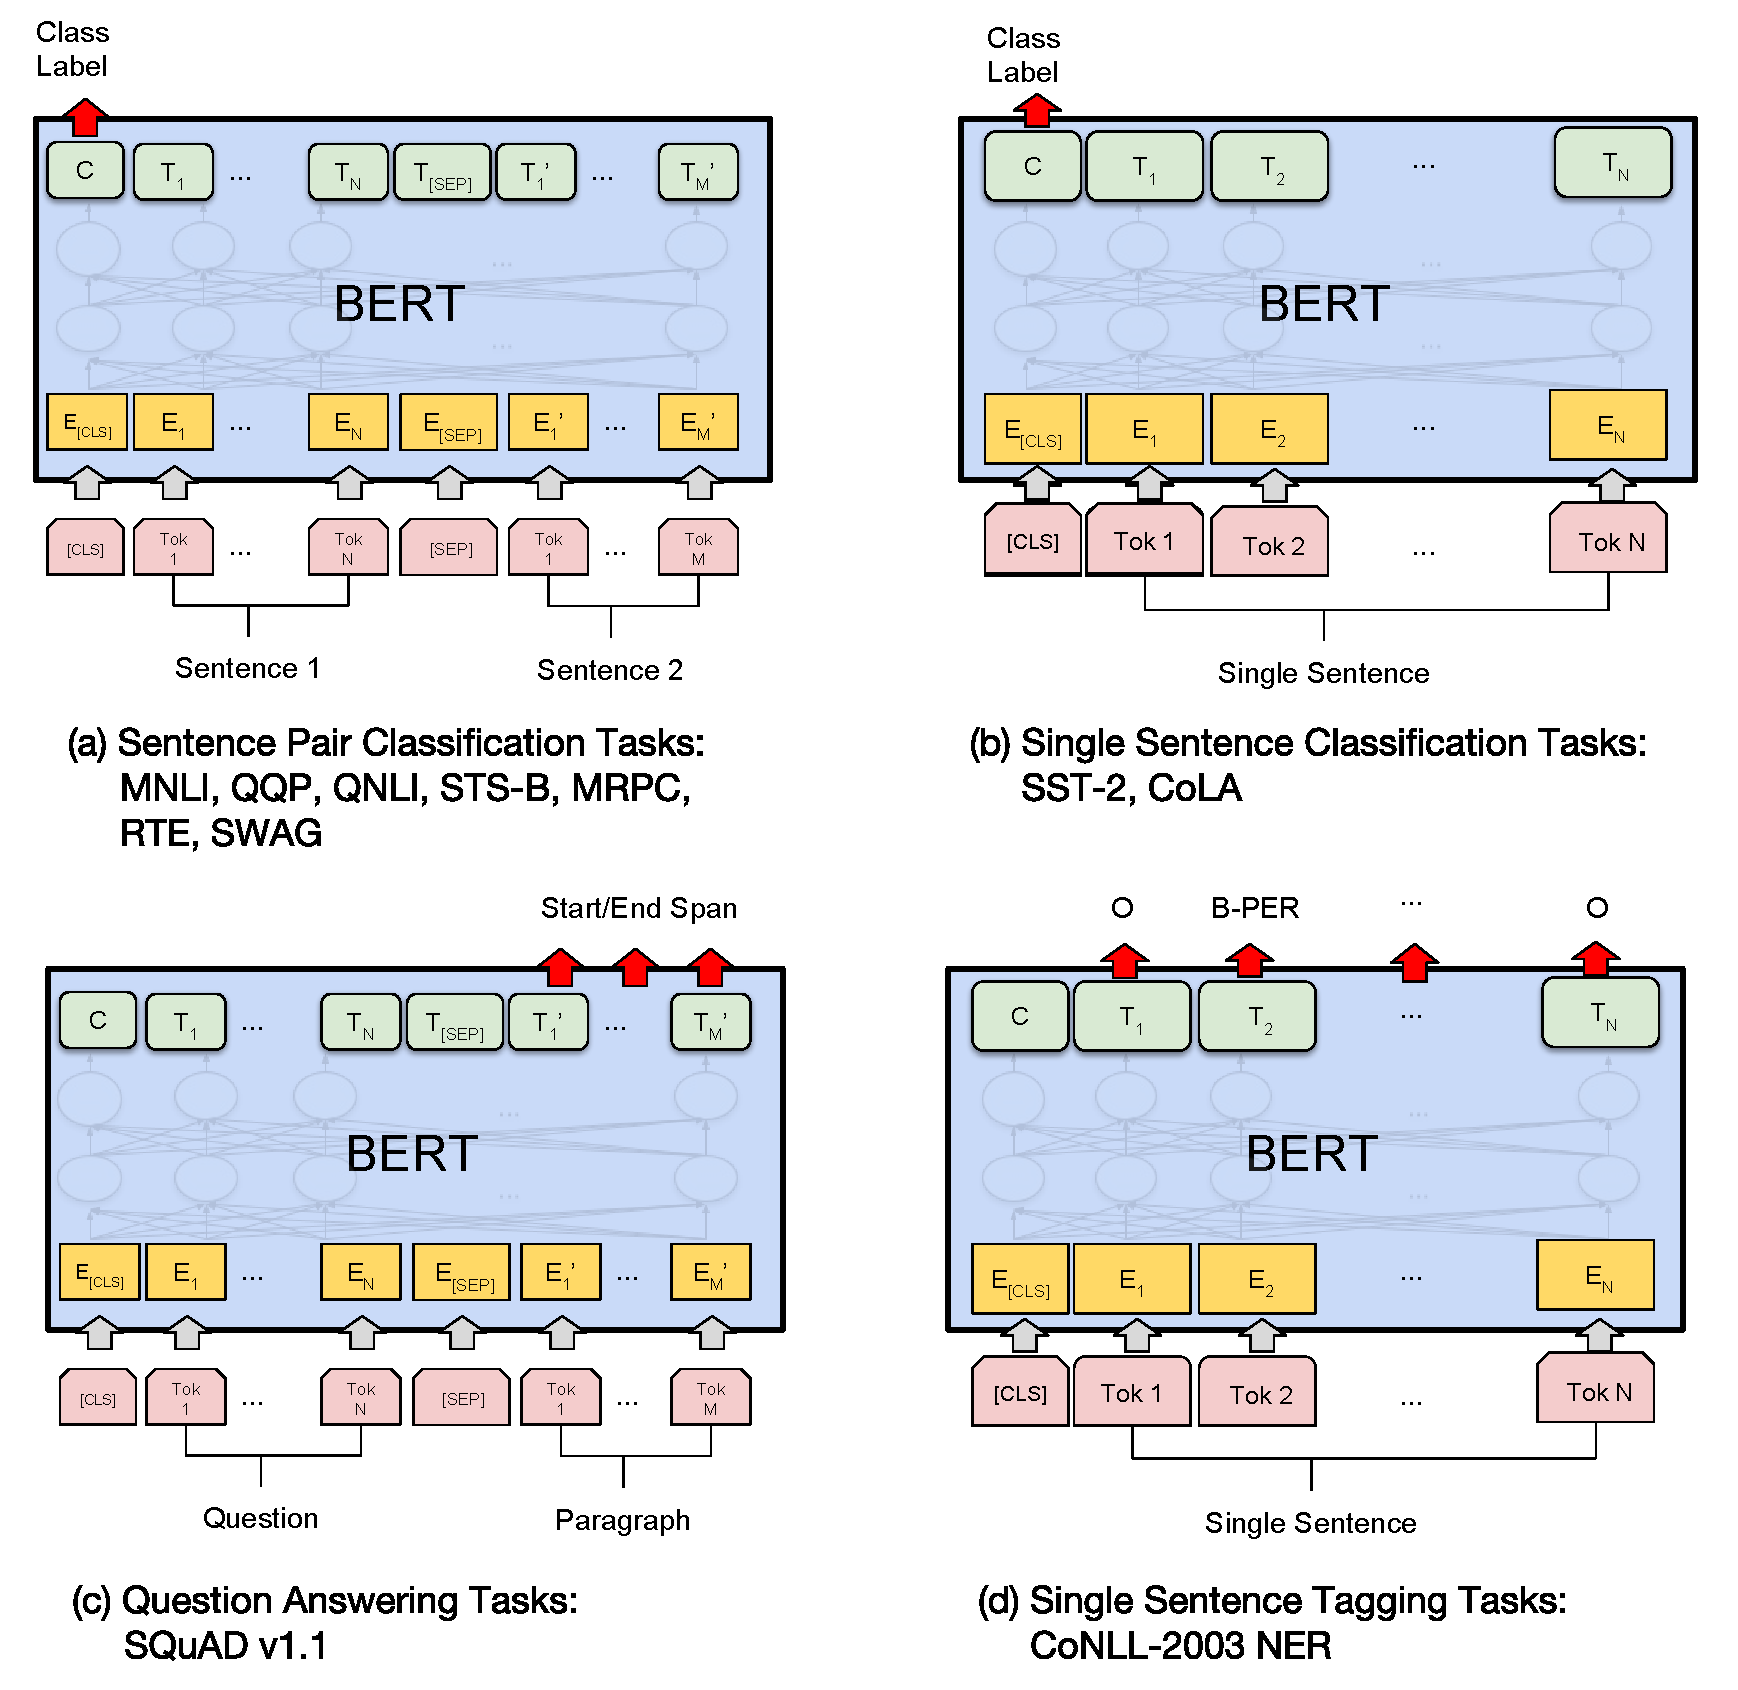
\includegraphics[width=0.90\textwidth]{figures/finetuning.pdf}
  \caption{\bert{} fine-tuning architectures for four task types.  (a)~Sentence-pair
           classification; (b)~single-sentence classification;
           (c)~extractive question answering; (d)~sequence labelling (NER).
           Only the top-layer head changes across tasks; the encoder is shared.}
  \label{fig:finetuning}
\end{figure}

\subsection{Practical Considerations}
\label{subsec:ft_practical}

\begin{itemize}
  \item \textbf{Learning rate warm-up.}  A linear warm-up over the first
        $10\%$ of training steps followed by linear decay is recommended to
        prevent catastrophic forgetting of pre-trained knowledge.
  \item \textbf{Batch size.}  Larger batch sizes (32--128) generally improve
        stability on small datasets; gradient accumulation can approximate large
        batches on memory-constrained hardware.
  \item \textbf{Layer-wise learning rate decay.}  Assigning lower learning rates
        to lower encoder layers and higher rates to the task head has been
        reported to improve fine-tuning stability~\cite{sun2019fine}.
\end{itemize}

% ============================================================
%  Section 7: Discussion and Impact
% ============================================================

\section{Discussion and Impact}
\label{sec:discussion}

\subsection{Key Contributions}
\label{subsec:contributions}

\bert{} introduced three innovations that, taken together, established a new paradigm
for NLP research and engineering:

\begin{enumerate}
  \item \textbf{Deep bidirectional pre-training.}  By employing the MLM objective,
        \bert{} learns representations that incorporate context from both directions
        simultaneously in every layer.  This is a departure from the shallow
        bidirectionality of ELMo (which concatenates unidirectional LMs) and from
        the strict left-to-right conditioning of GPT.

  \item \textbf{Unified pre-train–fine-tune framework.}  A single model can be
        adapted to diverse tasks --- classification, question answering, sequence
        labelling, semantic similarity --- with minimal architectural change,
        reducing the need for highly specialised task-specific designs.

  \item \textbf{State-of-the-art empirical results.}  Upon publication, \bert{}
        achieved new records on 11 NLP benchmarks, including a 7.7-point
        improvement on the GLUE benchmark~\cite{wang2018glue} and a 1.5 F1-point
        gain on SQuAD~v1.1~\cite{rajpurkar2016squad}.
\end{enumerate}

\subsection{Advantages}
\label{subsec:advantages}

\begin{itemize}
  \item \textbf{Strong transfer learning.}  Pre-trained \bert{} representations
        encode broad linguistic knowledge that transfers well to low-resource tasks
        where labelled data is scarce.

  \item \textbf{Task flexibility.}  The same encoder is applicable to sentence-level
        and token-level tasks without structural modification.

  \item \textbf{Contextual disambiguation.}  Because each token's representation
        is a function of all other tokens in the sequence, polysemous words are
        disambiguated naturally --- a capability absent from static embeddings.
\end{itemize}

\subsection{Limitations}
\label{subsec:limitations}

Despite its impact, \bert{} carries several notable limitations:

\begin{itemize}
  \item \textbf{Computational cost.}  Pre-training \bert{}-Large requires thousands
        of TPU hours and is prohibitively expensive for most academic and industrial
        teams without specialised hardware.  Inference latency is also high relative
        to simpler models, hampering deployment in latency-sensitive applications.

  \item \textbf{Fixed input length.}  The 512-token limit imposed by learned
        position embeddings makes \bert{} unsuitable for long documents without
        chunking heuristics.

  \item \textbf{NSP objective limitations.}  The NSP task does not require
        fine-grained linguistic understanding and can be learned by superficial
        topic-matching heuristics~\cite{liu2019roberta}.

  \item \textbf{Masked token proportion.}  Only 15\% of tokens are masked per
        step, yielding a sparse training signal relative to autoregressive models
        that compute loss over all tokens.

  \item \textbf{Discrepancy between pre-training and fine-tuning.}  The \mask{}
        token appears during pre-training but never during fine-tuning, creating a
        distribution mismatch that may degrade performance.
\end{itemize}

\subsection{Influence and Subsequent Work}
\label{subsec:subsequent}

\bert{}'s design has spawned a rich ecosystem of variants and successors, including:
\begin{table}[H]
  \centering
  \caption{\bert{} and contemporary models: a comparison of key properties.
           All models use the Transformer encoder architecture; differences lie in
           pre-training objectives, corpus size, and downstream performance.}
  \label{tab:model_comparison}
  \renewcommand{\arraystretch}{1.3}
  \begin{tabular}{lcccc}
    \toprule
    \textbf{Model} & \textbf{Type} & \textbf{Bidirectional} & \textbf{GLUE Score} & \textbf{Year} \\
    \midrule
    ELMo & Feature-based & Shallow & 76.2 & 2018 \\
    \bert{}-Base & Pre-train/Fine-tune & Yes (MLM) & 78.3 & 2018 \\
    GPT & Pre-train/Fine-tune & No (causal) & 72.3 & 2018 \\
    RoBERTa & Pre-train/Fine-tune & Yes (dynamic MLM) & 80.5 & 2019 \\
    ALBERT & Pre-train/Fine-tune & Yes (param. sharing) & 75.3 & 2019 \\
    \bottomrule
  \end{tabular}
\end{table}
\begin{itemize}
  \item \textbf{RoBERTa}~\cite{liu2019roberta}: removes NSP, trains with dynamic
        masking and larger batches, and demonstrates that pre-training for longer
        substantially improves performance.
  \item \textbf{ALBERT}~\cite{lan2019albert}: introduces parameter sharing across
        layers and factorised embedding parameterisation to reduce model size.
  \item \textbf{DistilBERT}~\cite{sanh2019distilbert}: uses knowledge distillation
        to produce a 40\%-smaller, 60\%-faster model retaining 97\% of \bert{}'s
        GLUE score.
  \item \textbf{Domain-specific BERTs}: BioBERT, SciBERT, ClinicalBERT, and others
        apply the same pre-training procedure to specialised corpora, demonstrating
        the generality of the framework.
\end{itemize}

\subsection{Conclusion}
\label{subsec:conclusion}

\bert{} marks a watershed moment in the evolution of NLP.  Its introduction of
deep bidirectional pre-training via masked language modelling demonstrated
conclusively that a single general-purpose encoder, pre-trained at scale, can
outperform highly engineered task-specific architectures across the full spectrum
of language understanding tasks.  The architectural and training insights embedded
in \bert{} continue to underpin state-of-the-art large language models, and its
influence on the field remains profound.


% ============================================================
%  Part 3: Applications, Limitations, and Legacy of BERT
% ============================================================

% ============================================================
%  Section: Applications of BERT
% ============================================================

\section{Applications of BERT}
\label{sec:applications}

One of \bert{}'s most significant contributions is the breadth and versatility of its
downstream applicability.  Because \bert{} is pre-trained once on massive corpora and
subsequently \emph{fine-tuned} with minimal task-specific supervision, a single
unified backbone can be adapted to a wide range of natural language processing tasks.
This section examines four representative application domains: sentiment analysis,
search intent understanding, question answering, and named entity recognition.

\subsection{Sentiment Analysis}
\label{subsec:sentiment}

Sentiment analysis---the task of classifying the emotional polarity of a piece of
text---is one of the most direct demonstrations of \bert{}'s text-classification
capability.  The input is formatted as a single sequence prefixed with the
\texttt{[CLS]} token and terminated with \texttt{[SEP]}; after fine-tuning, the
contextual representation of \texttt{[CLS]} is passed through a linear classification
head whose output dimension equals the number of sentiment classes.

Three representative examples illustrate the precision of \bert{}'s predictions.
A clearly positive review such as \emph{``I absolutely love the new product design!''}
yields a probability distribution strongly concentrated on the positive class
($P_{\text{Pos}} = 0.98$, $P_{\text{Neu}} = 0.015$, $P_{\text{Neg}} = 0.005$).
An ambiguous, informationally neutral query such as \emph{``how do I place orders''}
is correctly assigned to the neutral class ($P_{\text{Neu}} = 0.997$).  Conversely, an
implicitly negative statement such as \emph{``this is not the answer I was looking
for''} is classified as negative with high confidence ($P_{\text{Neg}} = 0.995$),
demonstrating \bert{}'s ability to capture negation through bidirectional context.
It is worth noting that \bert{}'s WordPiece tokenizer may segment rare words into
subword units prefixed with \texttt{\#\#}, but this has no adverse effect on
sentiment classification because contextual representations aggregate information
across the full token sequence~\cite{devlin2019bert}.

\subsection{Search Intent Understanding --- Google Search Integration}
\label{subsec:search}


\begin{figure}[H]
  \centering
  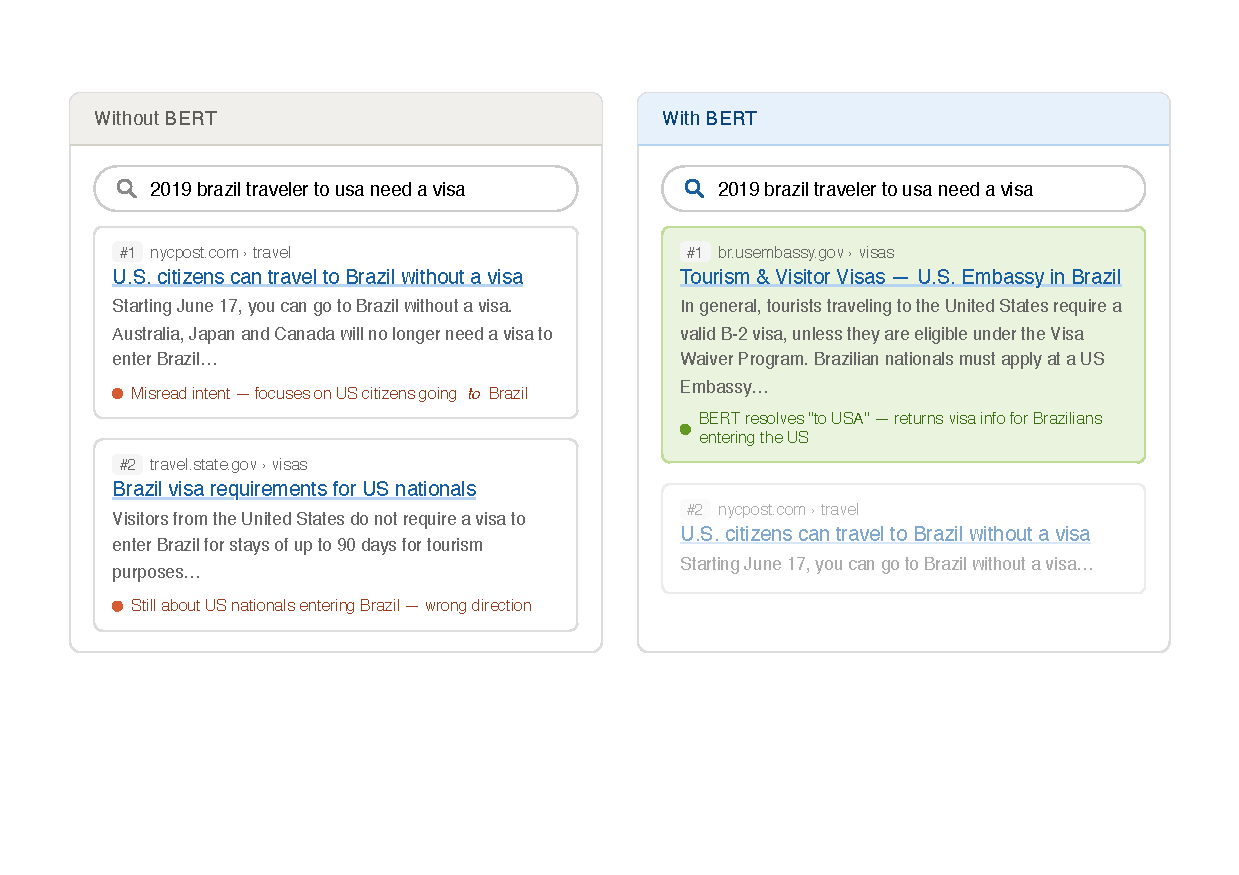
\includegraphics[trim=1cm 3.5cm 1cm 1.5cm, clip, width=0.90\textwidth]{figures/visa.pdf}
  \caption{\textbf{Impact of BERT on Search Intent Resolution.} The left panel (Without BERT) shows results focusing on U.S. citizens traveling \textit{to} Brazil, failing to capture the directional intent. The right panel (With BERT) correctly identifies the query ``2019 brazil traveler to usa'' as a request for U.S. entry requirements for Brazilian nationals.}
  \label{fig:visa-intent} % Changed to be unique and descriptive
\end{figure}

In October 2019, Google deployed \bert{} to improve the interpretation of natural
language search queries, affecting approximately one in ten English searches at
launch~\cite{nayak2019bert}.  The central challenge in web search is not merely
matching keywords but understanding the \emph{intent} embedded in a query, which
often hinges on subtle linguistic cues such as prepositions or word order.

Two canonical examples underscore this point.  For the query \emph{``2019 Brazil
traveler to USA need a visa''}, pre-\bert{} systems retrieved results focused on
US citizens travelling \emph{to} Brazil---misreading the directionality signalled by
the preposition \emph{to}.  After integrating \bert{}, the top result correctly
pointed to US Embassy visa requirements for Brazilian nationals, because \bert{}
conditions each token's representation on its full bilateral context and thus
correctly resolves the directional relationship.


\begin{figure}[H]
  \centering
  % trim= left bottom right top (adjust these values to zoom more/less)
  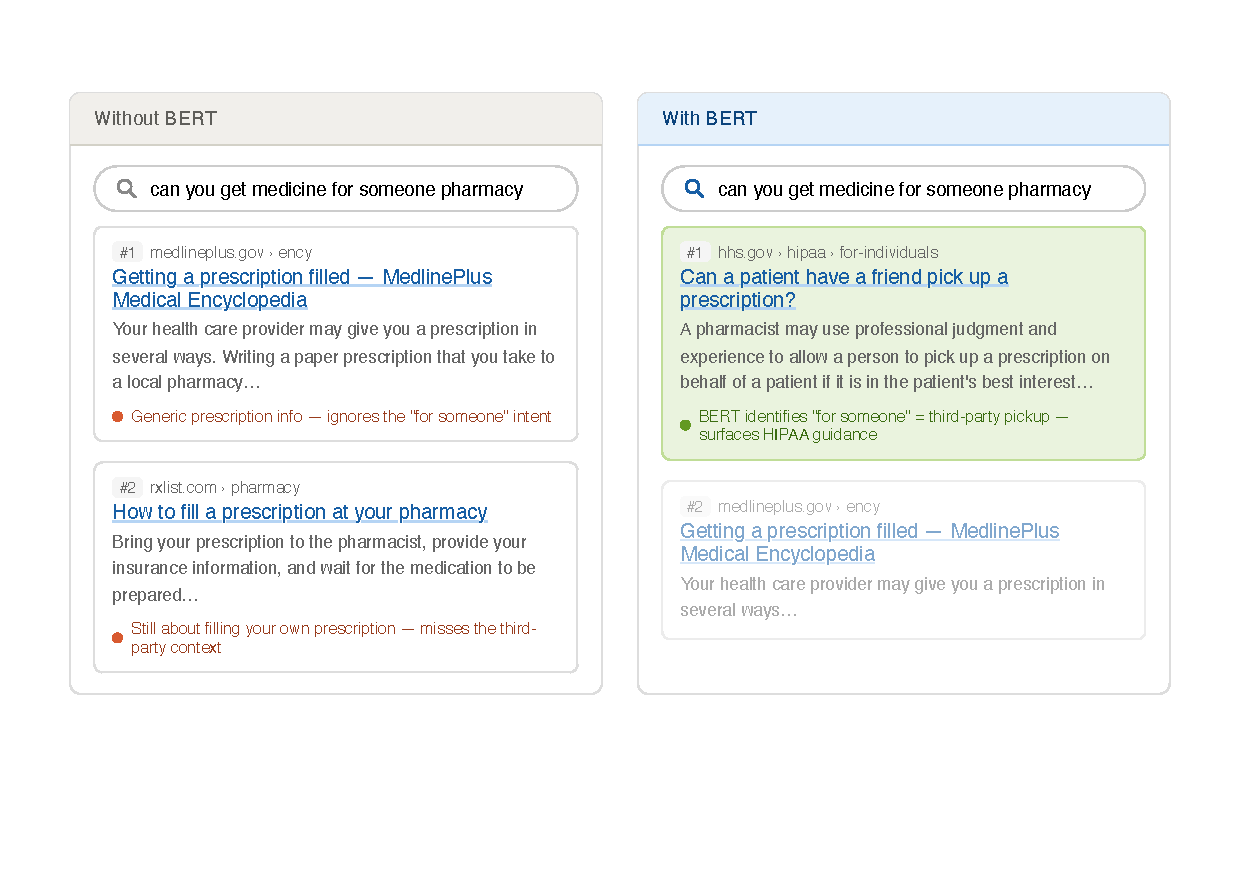
\includegraphics[trim=1cm 3cm 1cm 1.5cm, clip, width=0.90\textwidth]{figures/pharmacy.pdf}
  \caption{\textbf{Close-up of BERT Contextual Understanding.} Detailed view of the third-party intent resolution for pharmacy pickup queries.}
  \label{fig:pharmacy-zoom}
\end{figure}

A second example involves the query \emph{``Can you get medicine for someone
pharmacy''}.  Earlier systems surfaced general information about filling
prescriptions, overlooking the phrase \emph{``for someone''} which signals a
third-party pickup scenario.  \bert{}'s contextualisation correctly identifies
this intent, ranking results from authoritative health-policy sources that directly
address whether a pharmacist may dispense medication to a proxy.  These examples
demonstrate that even fine-grained syntactic relationships---which static keyword
matching cannot capture---are correctly resolved through \bert{}'s deep bidirectional
representations.

\subsection{Question Answering}
\label{subsec:qa}

Extractive question answering requires the model to locate a contiguous span of text
within a given passage that answers a posed question.  \bert{} addresses this as a
\emph{span extraction} task: the question and the context paragraph are concatenated
as \texttt{[CLS] Question [SEP] Context [SEP]}, and two linear layers predict the
start and end token indices of the answer span~\cite{devlin2019bert}.

Consider the following context passage: \emph{``The BERT-Large model is a powerhouse
of natural language processing.  It consists of 24 transformer layers and 16 attention
heads.  BERT-Large features 340 million parameters, allowing it to understand complex
nuances in human language.''}  Given the question \emph{``How many parameters does
BERT-Large have?''}, \bert{} assigns the highest start-position probability to the
token \emph{340} and the highest end-position probability to the token
\emph{million}, extracting the correct answer span \emph{``340 million''}.  This
behaviour arises because the cross-attention between the question tokens and the
context tokens guides the model towards the semantically relevant passage fragment.
On the Stanford Question Answering Dataset~(SQuAD~2.0), \bert{} achieved
state-of-the-art performance at the time of publication, surpassing human-level
accuracy on the held-out test set~\cite{rajpurkar2018know}.

\subsection{Named Entity Recognition}
\label{subsec:ner}

\begin{figure}[H]
  \centering
  % trim= left bottom right top 
  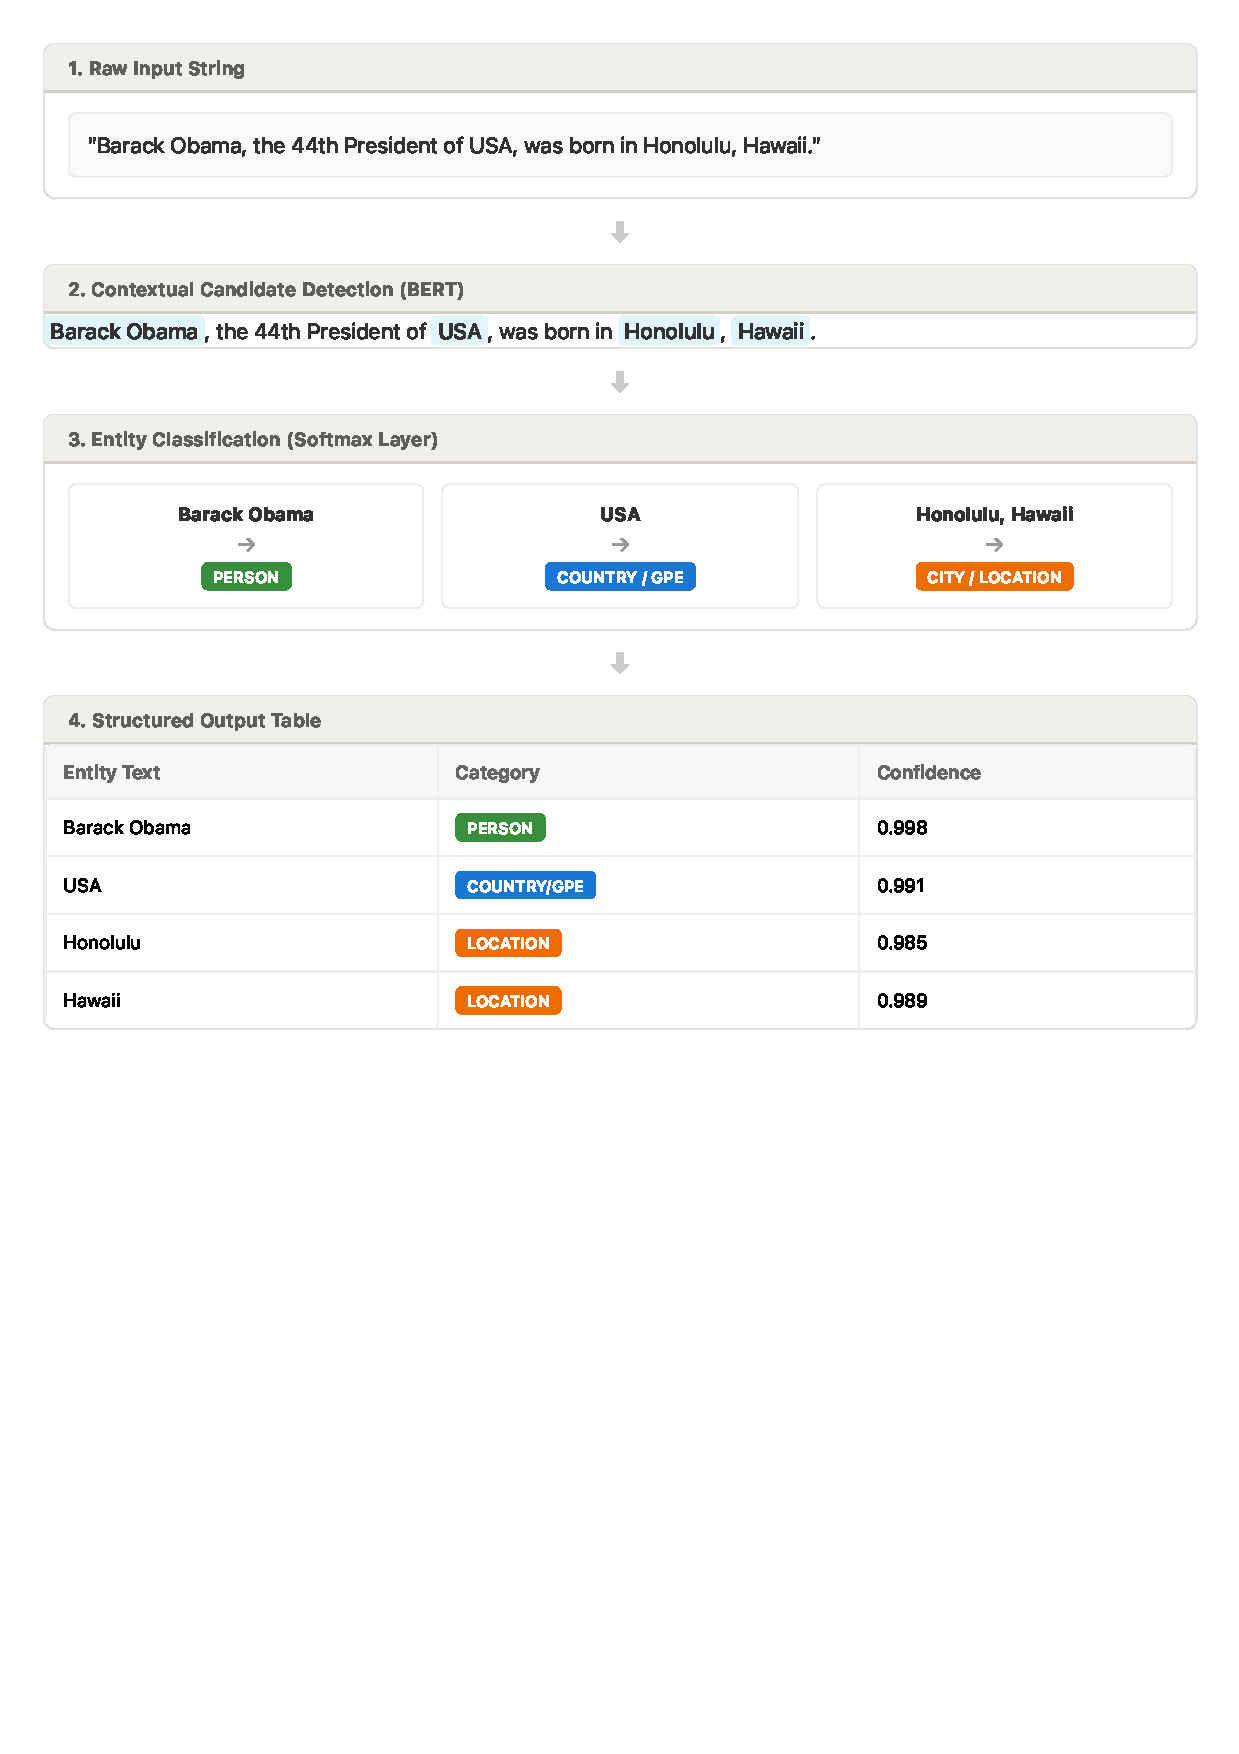
\includegraphics[trim=0cm 11cm 0cm 0.5cm, clip, width=0.90\textwidth]{figures/nerPipeline.pdf}
  \caption{\textbf{Four-Stage Named Entity Recognition (NER) Pipeline.} The diagram illustrates the transition from (1)~raw input strings to (2)~contextual candidate detection via \bert{}, followed by (3)~token-level classification into categories such as \textbf{Person}, \textbf{GPE}, and \textbf{Location}, and finally (4)~the consolidation of labels into a structured output table.}
  \label{fig:ner-pipeline-stages}
\end{figure}

Named Entity Recognition~(NER) is a token-level sequence labelling task in which the
model assigns a category label to each token in a sentence.  Common entity categories
include Person, Organisation, Location, Geopolitical Entity~(GPE), and Date/Time
expressions.  \bert{} approaches NER by appending a token-level classification head
atop the contextual encoder; the representation of each subword token is independently
passed through a softmax layer to produce a label~\cite{devlin2019bert}.

The pipeline can be described in four stages.  First, the raw input string---for
example, \emph{``Barack Obama, the 44th President of USA, was born in Honolulu,
Hawaii.''}---is tokenised and fed to the encoder.  Second, the model exploits
contextual signals to identify candidate entities; the phrase \emph{Barack Obama}
is highlighted as a named entity by virtue of its proper-noun characteristics and
surrounding syntactic structure.  Third, each detected entity is assigned its most
probable label: \emph{Barack Obama} $\rightarrow$ \textbf{Person}, \emph{USA}
$\rightarrow$ \textbf{Country/GPE}, and \emph{Honolulu, Hawaii} $\rightarrow$
\textbf{City/Location}.  Fourth, the labelled entities are collated into a structured
output table, which downstream applications can directly consume for information
extraction or knowledge-graph construction.


% ============================================================
%  Section: Limitations of BERT
% ============================================================

\section{Limitations of BERT}
\label{sec:limitations}

Despite its transformative impact, \bert{} is not without significant limitations.
Understanding these shortcomings is essential both for deploying \bert{} responsibly
and for motivating the extensive body of successor work that followed its
release~\cite{rogers2020primer}.


\begin{figure}[H]
  \centering
  % trim= left bottom right top 
  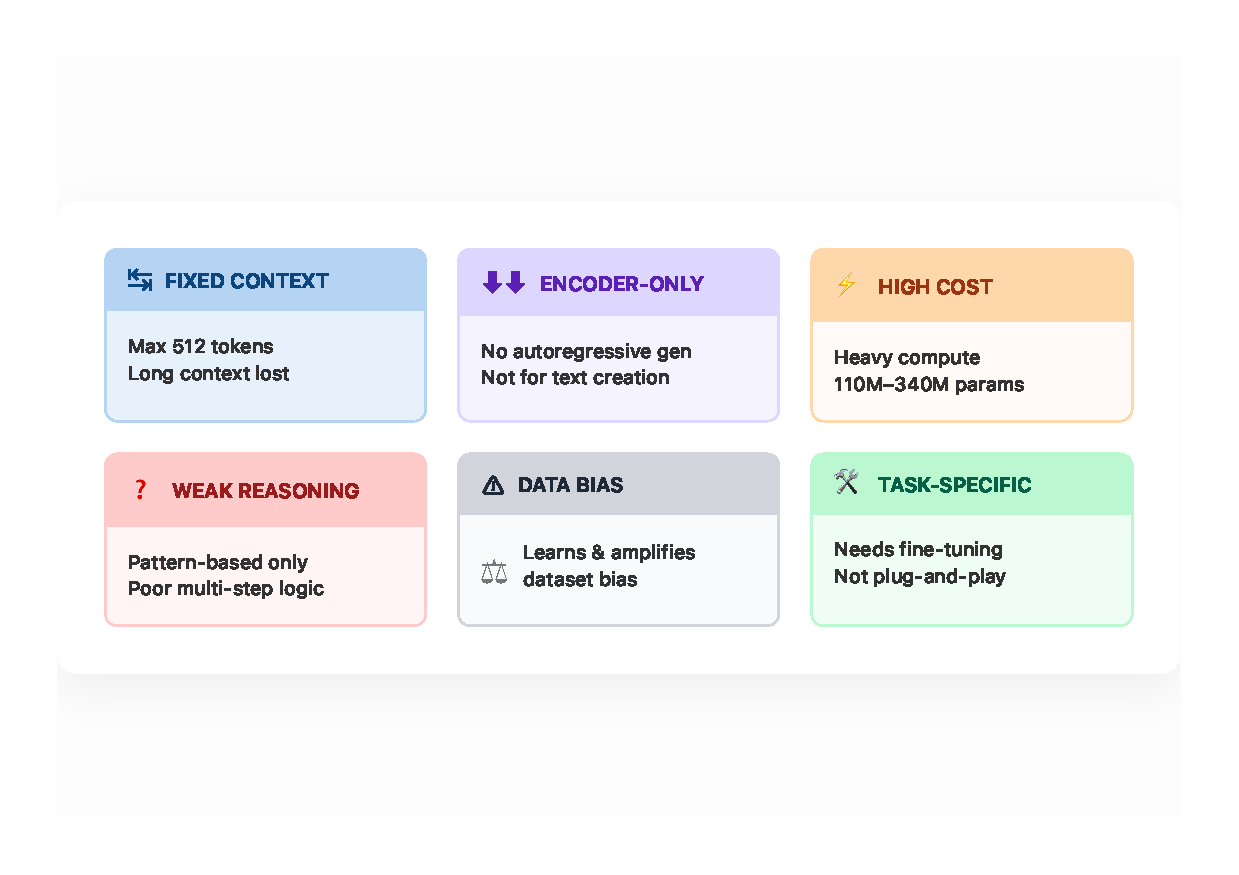
\includegraphics[trim=1cm 3cm 1cm 4cm, clip, width=0.90\textwidth]{figures/limitation.pdf}
  \caption{\textbf{Limitations of BERT.} Fixed context window, encoder-only design, high computational cost, weak reasoning ability, inherited data bias, and dependence on task-specific fine-tuning.}
  \label{fig:bert-limitations}

\end{figure}


\begin{enumerate}
  \item \textbf{Fixed context window.}  \bert{} operates on sequences of at most
        512 tokens.  Documents exceeding this limit must be truncated or chunked,
        which breaks cross-segment dependencies and can degrade performance on
        long-document tasks such as legal contract analysis or scientific paper
        summarisation.

  \item \textbf{Encoder-only architecture---no text generation.}  Because \bert{}
        is a \emph{bidirectional encoder}, it is architecturally incapable of
        auto-regressively generating text.  Tasks requiring open-ended generation,
        such as machine translation, abstractive summarisation, or dialogue,
        require decoder-equipped architectures (e.g., GPT, T5,
        BART)~\cite{lewis2019bart}.

  \item \textbf{Computational cost.}  \bert{}-Base contains 110 million parameters
        and \bert{}-Large 340 million.  Both require substantial GPU memory and
        inference time, making real-time deployment in resource-constrained
        environments (e.g., on-device mobile applications) challenging without
        additional compression~\cite{sanh2019distilbert}.

  \item \textbf{Limited commonsense and logical reasoning.}  \bert{}'s pre-training
        objectives---Masked Language Modelling and Next Sentence Prediction---equip
        it with strong distributional semantics but do not explicitly train it to
        perform multi-step reasoning or apply world knowledge consistently.  This
        manifests as errors on tasks requiring numerical reasoning, causal inference,
        or structured commonsense knowledge~\cite{rogers2020primer}.

  \item \textbf{Inherited data bias.}  \bert{} is pre-trained on BookCorpus and
        English Wikipedia.  These corpora encode various societal biases pertaining
        to gender, race, and cultural perspective.  Studies have shown that \bert{}'s
        representations reflect and can amplify such biases, which raises ethical
        concerns in applications involving hiring, credit scoring, or content
        moderation~\cite{bender2021dangers}.
\item \textbf{Task-specific dependency.} \bert{} is not a general-purpose, out-of-the-box 
        solution. Its pre-training objective (masked language modeling) does not directly 
        align with most downstream tasks, requiring additional fine-tuning on labeled data 
        for each specific application. As a result, performance is highly dependent on 
        task-specific datasets and supervision, limiting transferability and increasing 
        deployment cost.
\end{enumerate}


% ============================================================
%  Section: What Came After BERT
% ============================================================

\section{What Came After BERT}
\label{sec:successors}

\bert{}'s introduction triggered an era of rapid architectural innovation aimed at
addressing each of its known limitations while preserving or extending its core
strengths.  The resulting family of models can be broadly categorised into three
groups: training-efficiency improvements, context and modelling extensions, and
deployment-friendly distillations.

\begin{figure}[H]
  \centering
  % trim= left bottom right top 
  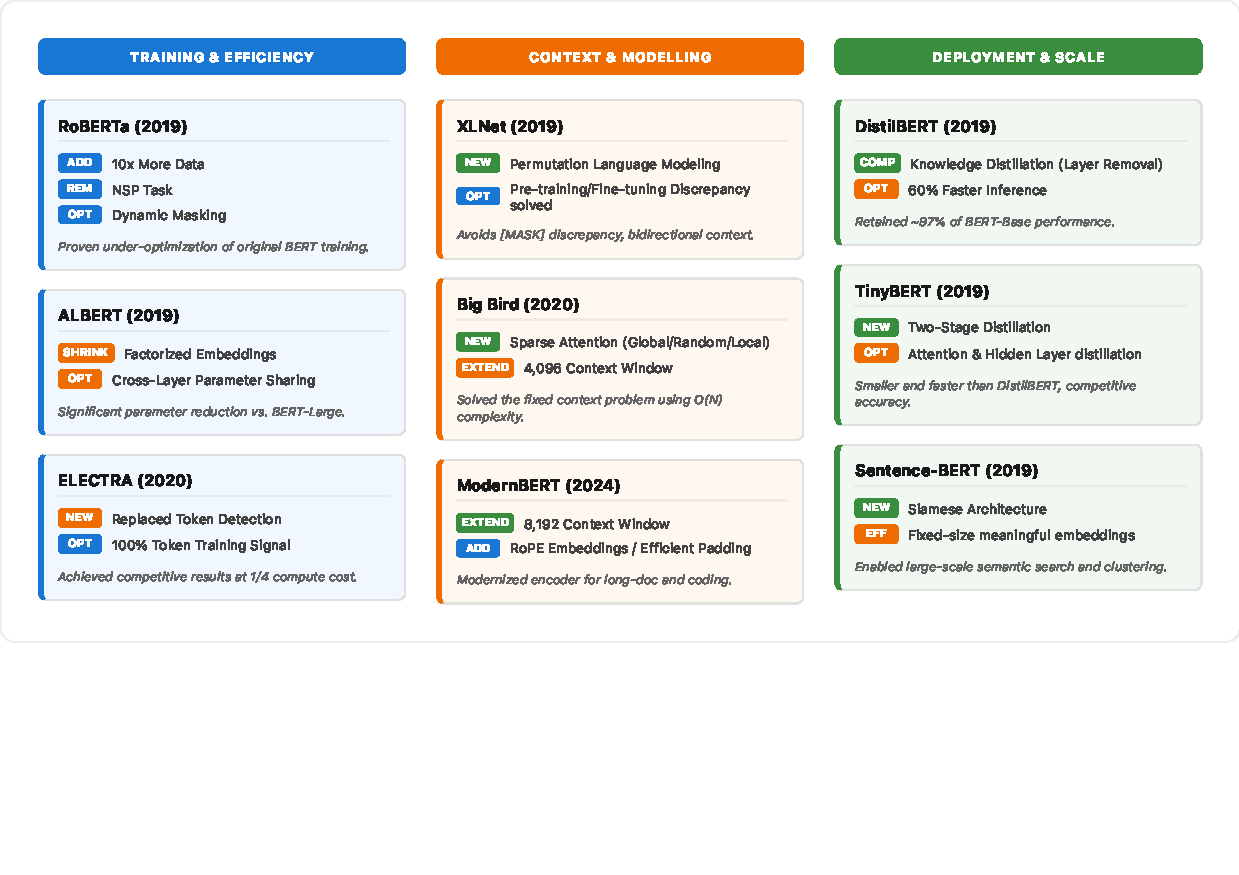
\includegraphics[trim=0cm 3cm 0cm 0cm, clip, width=0.90\textwidth]{figures/successors.pdf}
  \caption{\textbf{BERT Successors and Improvements.} Overview of key BERT-based models that address limitations in pre-training, model efficiency, context length, reasoning, and task adaptability.}
  \label{fig:bert-succesors}
\end{figure}

\subsection{Training and Efficiency Improvements}
\label{subsec:training-successors}

\textbf{RoBERTa}~(Robustly Optimised BERT Pre-training Approach, 2019) demonstrated
that \bert{}'s original training was substantially under-optimised.  By training on
ten times more data, removing the Next Sentence Prediction objective, and adopting
\emph{dynamic masking} (so that each training pass sees a different random mask),
Liu et al.\ achieved consistent improvements across all \textsc{GLUE} benchmarks
without any architectural change~\cite{liu2019roberta}.


\textbf{ALBERT}~(A Lite BERT, 2019) introduced two parameter-reduction techniques:
\emph{factorised embedding parameterisation}, which decouples the vocabulary
embedding size from the hidden layer size, and \emph{cross-layer parameter sharing},
where all Transformer layers share identical weights.  These changes reduced the
parameter count by up to 89\% relative to \bert{}-Large while maintaining competitive
accuracy~\cite{lan2019albert}.

\textbf{ELECTRA}~(Efficiently Learning an Encoder that Classifies Token Replacements
Accurately, 2020) replaced the MLM objective with a more sample-efficient
\emph{replaced-token detection} pre-training signal: a small generator network
corrupts the input and the main discriminator learns to identify which tokens were
replaced.  Because every token contributes a training signal (rather than only the
15\% masked tokens in standard MLM), ELECTRA reached \bert{}'s performance with
substantially less compute~\cite{clark2020electra}.

\subsection{Context and Modelling Extensions}
\label{subsec:context-successors}

\textbf{XLNet}~(2019) abandoned the masked-token paradigm in favour of
\emph{permutation language modelling}: by training the model to predict tokens in all
possible orderings of the input sequence, XLNet obtains bidirectional context without
the train--inference discrepancy introduced by \texttt{[MASK]}
tokens~\cite{yang2019xlnet}.


\textbf{BigBird}~(2020) introduced sparse attention mechanisms combining global, 
local, and random attention patterns to extend BERT's context window up to 4,096 
tokens while maintaining linear computational complexity. This design addresses 
BERT's fixed-context limitation, making it effective for long-document understanding 
and retrieval tasks~\cite{zaheer2020bigbird}.


\textbf{ModernBERT}~(2024) extended the context window to 8\,192 tokens through
Rotary Position Embeddings~(RoPE), incorporated efficient padding removal to avoid
unnecessary computation on padding tokens, and updated the architectural components
with current best practices.  These changes make ModernBERT competitive on long-document
retrieval and coding tasks while retaining the familiar encoder-only
paradigm~\cite{modernbert2024}.

\subsection{Deployment-Friendly Models}
\label{subsec:lightweight-successors}

\textbf{DistilBERT}~(2019) applied \emph{knowledge distillation} to compress
\bert{}-Base into a model with 40\% fewer parameters and 60\% faster inference,
retaining approximately 97\% of \bert{}'s performance on downstream
benchmarks~\cite{sanh2019distilbert}.

\textbf{TinyBERT}~(2019) applied a two-stage knowledge distillation approach 
to compress BERT into a smaller, faster model. By distilling both attention 
and hidden layers from the teacher model, TinyBERT achieves competitive 
accuracy with reduced parameters and inference time, enabling deployment 
in resource-constrained environments~\cite{jiao2019tinybert}.


\textbf{Sentence-BERT}~(SBERT, 2019) fine-tuned \bert{} with a Siamese network
architecture and a contrastive objective, producing \emph{fixed-size sentence
embeddings} that are semantically meaningful under cosine similarity.  This allows
large-scale semantic textual similarity, clustering, and information retrieval tasks
to be performed efficiently without the expensive cross-encoder inference required by
vanilla \bert{}~\cite{reimers2019sentencebert}.


% ============================================================
%  Section: Conclusion
% ============================================================

\section{Conclusion}
\label{sec:conclusion}

\bert{} represents a watershed moment in the history of natural language processing.
By introducing deep bidirectional pre-training via the Masked Language Model
objective, it resolved the fundamental limitation of unidirectional context that
constrained all prior pre-trained representations.  Its unified \emph{pre-train then
fine-tune} paradigm eliminated the need to design task-specific architectures from
scratch, establishing a blueprint that the entire field subsequently
adopted~\cite{devlin2019bert}.

Table~\ref{tab:before-after-bert} summarises the principal qualitative shifts that
\bert{} introduced, contrasting the capabilities of the NLP landscape before and
after its release.

\begin{table}[ht]
\centering
\caption{The evolution of NLP capabilities introduced by \bert{}.}
\label{tab:before-after-bert}
\renewcommand{\arraystretch}{1.4}
\begin{tabular}{p{0.44\textwidth} p{0.44\textwidth}}
\hline
\textbf{Before BERT} & \textbf{After BERT} \\ \hline
Unidirectional context (LSTMs, ELMo) & Full bidirectional context \\
Separate model trained per task & One backbone, many tasks \\
Shallow contextual signals & Deep contextual embeddings \\
Expensive training for each new task & Efficient fine-tuning on small data \\
Sequential processing (slow) & Parallel Transformer layers (fast) \\ \hline
\end{tabular}
\end{table}

The legacy of \bert{} extends far beyond its benchmark scores.  From its release in
2018 through RoBERTa and ALBERT in 2019, ELECTRA in 2020, and ModernBERT in 2022,
each successive model refined or extended \bert{}'s core ideas, collectively pushing
the frontier of language understanding.  Today, \bert{} and its successors underpin
production systems for web search, question answering, document classification, and
information extraction at global scale.  More broadly, \bert{} established the
Transformer encoder as the canonical architecture for language understanding---a
position it continues to hold, and one that has influenced the design of every major
language model released since~\cite{rogers2020primer, bender2021dangers}.

% ---- Bibliography --------------------------------------------
\newpage
\printbibliography[heading=bibintoc, title={References}]

\end{document}
